\documentclass[numbers, 10pt, preprint]{sigplanconf}
%\documentclass[10pt]{sigalternate052015}

\usepackage{amsmath}
\usepackage{amssymb}
\usepackage{xcolor}
\usepackage{url}
\usepackage{times}
\usepackage{xspace}
\usepackage{listings}
\usepackage{code}
\usepackage{algorithm}
\usepackage[noend]{algpseudocode}
\usepackage{tikz}
\usetikzlibrary{arrows,automata,positioning}
\let\proof\relax
\let\endproof\relax
\usepackage{amsthm}
\usepackage{subcaption}
\usepackage{balance}
\usepackage[ampersand]{easylist}
\usepackage{textcomp}
\usepackage{enumitem}
\usepackage{pifont}
\newcommand{\cmark}{\ding{51}}
\newcommand{\xmark}{\ding{55}}

\definecolor{princetonorange}{RGB}{255,143,0}
\definecolor{tmlblue}{RGB}{0,58,120}  % tmlblue == Toronto Maple Leafs Blue!

\newcommand{\todo}[1]{\textcolor{red}{[TODO: #1]}}
\newcommand{\ratul}[1]{\textcolor{blue}{[ratul: #1]}}
\newcommand{\ryan}[1]{\textcolor{green}{[ryan: #1]}}
\newcommand{\dpw}[1]{\textcolor{tmlblue}{[dpw: #1]}}
\newcommand{\todd}[1]{\textcolor{princetonorange}{[todd: #1]}}

\newcommand{\EG}{\emph{e.g.}}
\newcommand{\IE}{\emph{i.e.}}
\newcommand{\ETC}{\emph{etc.}}
\newcommand{\ETAL}{\emph{et al.}}

\newcommand{\sysname}{{\small \sf Methane}\xspace}
\newcommand{\sysnamesec}{{\sf Methane}\xspace}
\newcommand{\propane}{{\small \sf Propane}\xspace}

\newcommand{\para}[1]{\paragraph*{\textbf{#1}}}

\newcommand{\set}[1]{\ensuremath{\{ #1 \} }}
\newcommand{\abs}[1]{\ensuremath{ \lvert #1 \rvert }}

\newcommand{\CD}[1]{\texttt{\small #1}}  % code font
\newcommand{\KW}[1]{\texttt{\small\bfseries{#1}}}

\newcommand{\True}{\CD{true}}
\newcommand{\Define}{\KW{define}}
\newcommand{\Prefer}{\texttt{>>}}
\newcommand{\Path}{\texttt{=>}}
\newcommand{\Link}{\texttt{->}}
\newcommand{\Agg}{\KW{agg}}
\newcommand{\Any}{\KW{any}}
\newcommand{\None}{\KW{drop}}
\newcommand{\In}{\KW{in}}
\newcommand{\Out}{\KW{out}}
\newcommand{\AND}{\texttt{\&}}
\newcommand{\OR}{\texttt{|}}
\newcommand{\NOT}{\texttt{!}}
\newcommand{\Intersect}{\ensuremath{\cap}}
\newcommand{\Union}{\ensuremath{\cup}}

\newcommand{\Exit}{\KW{exit}}
\newcommand{\End}{\KW{end}}
\newcommand{\Start}{\KW{start}}
\newcommand{\Enter}{\KW{enter}}
\newcommand{\Eventually}{\KW{eventually}}
\newcommand{\Already}{\KW{already}}
\newcommand{\Internal}{\KW{internal}}
\newcommand{\Never}{\KW{never}}
\newcommand{\Always}{\KW{always}}
\newcommand{\Through}{\KW{through}}
\newcommand{\LinkKW}{\KW{link}}
\newcommand{\PathKW}{\KW{path}}
\newcommand{\Novalley}{\KW{novalley}}

\renewcommand{\path}[2]{ #1 \mapsto \ensuremath{#2} }

%% grammar
\newcommand{\BNFALT}{\;\;|\;\;}
\newcommand{\hdr}[2]{\flushleft \chdr{\hspace{5mm}#1}{#2}}
\newcommand{\chdr}[2]{\textbf{#1} {#2} \\ \centering}%

\newtheorem{thm}{Theorem}
\newtheorem{defn}{Definition}
\newtheorem{lem}[thm]{Lemma}

\begin{document}

%\CopyrightYear{2016}
%\setcopyright{acmcopyright}
%\conferenceinfo{SIGCOMM '16,}{August 22-26, 2016, Florianopolis , Brazil}
%\isbn{978-1-4503-4193-6/16/08}\acmPrice{\$15.00}
%\doi{http://dx.doi.org/10.1145/2934872.2934909}

\special{papersize=8.5in,11in}
\setlength{\pdfpageheight}{\paperheight}
\setlength{\pdfpagewidth}{\paperwidth}

\conferenceinfo{CONF 'yy}{Month d--d, 20yy, City, ST, Country}
\copyrightyear{20yy}
\copyrightdata{978-1-nnnn-nnnn-n/yy/mm}
\copyrightdoi{nnnnnnn.nnnnnnn}

\titlebanner{DRAFT -- do not distribute}        % These are ignored unless
\preprintfooter{submission for PLDI 2017}   % 'preprint' option specified.

\title{Network Configuration Synthesis with Abstract Topologies}

%\author{Paper \#324, 14 pages}

%\authorinfo{Ryan Beckett \and David Walker}{Princeton}{}
%\authorinfo{Ratul Mahajan \and Jitendra Padhye}{Microsoft}{}
%\authorinfo{Todd Millstein}{UCLA}{}

\authorinfo{}{}{}

%\author{%
%Ryan Beckett\\
%  \affaddr{Princeton}
%  %\\
%  %\email{rbeckett@princeton.edu}
%\and
%Ratul Mahajan\\
%  \affaddr{Microsoft}
%  %\\
%  %\email{ratul@microsoft.com}
%\and
%Todd Millstein\\
%  \affaddr{UCLA}
%  %\affaddr{University of California, Los Angeles}
%  %\\
%  %\email{todd@cs.ucla.edu}
%\and
%Jitendra Padhye\\
%  \affaddr{Microsoft}
%  %\\
%  %\email{padhye@microsoft.com}
%\and
%David Walker\\
%  \affaddr{Princeton}
%  %\\
%  %\email{dpw@princeton.edu}
%}

\maketitle


%=====================================================
%
%
%  **Abstract**
%
%
%=====================================================


% Points to make
%
% (1) Lets operators think about topologies/policies at a high-level of abstraction
%     - matches current thinking (e.g., templates)
%
% (2) Promotes a correct-by-construction methodology
%
%     properties that hold over abstract topologies hold over concrete ones
%      - includes correct forwarding behavior
%      - includes reachability (under k-failures)
%
% (3) Enables reusability (e.g., across datacenters) and expansion (e.g., within a datacenter)
%
% (4) lets us scale synthesis to large-scale topologies

\textbf{Abstract---}
We develop techniques for automated reasoning about end-to-end properties of
abstract network topologies, and embody them in a network synthesis tool called
\sysname. \sysname allows network operators to write a high-level routing policy
over an abstraction of their network topology. From such a specification,
\sysname synthesizes a collection of router configurations running the
distributed Border Gateway Protocol (BGP) that are guaranteed to implement the
centralized routing policy for any concrete instantiation of the abstract
topology, and for any combination of network failures in the resulting concrete
topology.
%
Additionally, properties proven by \sysname over the abstract topology, such as
reachability between a source and destination under k-failures, are also
guaranteed to hold under any concrete instantiation of the abstract topology.
%
Something something, expandable/incremental networks. Something something scales
compilation to large networks. Something something, templates easier to
understand.
%These strong guarantees allow operators to reason about the routing behavior of
%their network at a high-level abstraction, while also generating an efficient
%low-level implementation.
%
%In addition, operators are able to safely change or expand their network in any
%way, so long as the new resulting topology also respects the abstraction.
%
We test \sysname out on ... blah blah blah



%=====================================================
%
%
%  **Keywords**
%
%
%=====================================================

%\vspace{0.1in} \noindent \textbf{CCS Concepts}\\ $\bullet$ Networks
%$\rightarrow$ {\em Network control algorithms; Network reliability; Network
%management;} $\bullet$ Software and its engineering $\rightarrow$ {\em
%Automated static analysis; Domain specific languages}

%\vspace{0.1in} \noindent \textbf{Keywords}\\ Propane; Domain-specific Language;
%BGP; Synthesis; Compilation; Fault Tolerance; Distributed Systems


%=====================================================
%
%
%  **Introduction**
%
%
%=====================================================

\section{Introduction} \label{sec:introduction}


% Hence, one approach to improving network reliability is to develop better
% languages for network configuration.  Such languages should be defined at a
% higher level of abstraction than existing configuration languages and provide
% support built-in support for verification of important properties, thereby
% avoiding entire classes of configuration errors automatically.

%An important class of networks are the large \emph{structured networks}
%commonly deployed in industrial data centers.

Computer networks run many critical services, and every second of downtime is
costly at best and dangerous at worst.  Keeping these complex systems up and
running 24/7 is an enormous
challenge~\cite{mahajan+:bgp-misconfiguration,feamster+:rcc,batfish,dc-failure-study}.
%
While hardware faults, backhoes, power failures and natural disasters all pose
problems, studies have consistently shown that human error in network
configuration is one of the leading cause of network
outages~\cite{juniper-study,xx}.

To manage and configure large networks today, instead of considering individual
devices, operators classify devices devices into {\em roles}. A role refers to
specific functionality and is played by one or more devices. For instance, in a
data center, roles may correspond to "top-of-rack," "aggregation," and "spine"
routers; and in a backbone network, they may correspond to "core" and "border"
routers. While the network may have hundreds or thousands of devices---a scale
that is impossible for humans to handle---there tend to be a handful of roles.
%
Operators author a configuration {\em template} for each role. Templates are
macros that can be instantiated with different concrete values, based on the
network topology, to generate a configuration for each device.

Unfortunately, template construction is a low-level, manual process. Operators
manually decompose network-wide routing and fault-tolerance policies (e.g.,
prefer one end-to-end path over another or no loss in connectivity after any
one-link failure) across roles and encode them using assembly-language-like
configuration primitives (e.g., role A should not transmit routing information
from B to C). Such decomposition tasks are highly complex~\cite{propane}.

Worse, operators can never be sure that the generated templates correctly
implement the policy,  beyond testing some concrete instantiations using
simulation or verification tools~\cite{x,y}. Testing based on concrete
instantiations is insufficient because large networks evolve continuously, as
devices and links are added or taken offline for maintenance. Templates that
work for the current network topology, may or may not work for future
topologies. Updating the templates, if found to not work for a future topology,
may cause trickle-down, network-wide configuration changes, which is highly
disruptive. Building sophisticated tools for validating templates is difficult
because the templates today have no particular semantics---which policies they
implement and for which topologies---other than the semantics of the
configurations that one obtains from instantiating them.

%It is no wonder that a major
%network outage, such as the one that grounded all United Air flights
%in July 2015~\cite{x}, makes international news every few months.

Given the challenges of generating and validating network configurations, one
might think that operators will be receptive to systems that can generate
provably-correct configurations from high-level policy
specifications~\cite{x,y,z,configassure,propane}. However, our conversations
with two major cloud providers reveal that operators of large networks are
reluctant to use such systems. While they think of their network abstractly, in
terms of roles, these systems require concrete topologies, with no understanding
of roles as a first-order abstraction.  Even if two devices play the same role,
there is no guarantee that the systems will generate (syntactically) similar
configurations; if the operators want to debug or analyze system output, they
will have to consider hundreds of device configurations instead of a handful of
role configurations. These systems become even more brittle when the network
evolves. Any change in network topology requires re-execution of the engine,
from scratch, on the changed topology.  The result may be a completely different
set of configurations.

We present \sysname, a system to generate provably-correct role templates. It
allows operators to input \emph{abstract network topologies} in terms of roles
and their connectivity. For instance, they may specify roles for ``top-of-rack''
and ``aggregation" routers and specify that every top-of-rack router connects to
at least two aggregation routers (to tolerate the failure of a link to an
aggregation router). Other inputs to \sysname include the routing policy of the
network and its fault-tolerance requirements (e.g., the number of link failures
to tolerate). For routing policy, we borrow notation from
Propane~\cite{propane},  which specifies traffic paths at a high-level of
abstraction. But while Propane policies refer to concrete devices, \sysname
policies refer to abstract roles.

Based on these inputs, the \sysname compiler generates one template per role. It
guarantees that, when the templates are instantiated to configurations for {\em
any} concrete topology that complies with the abstract topology, the result
network will correctly implement the routing policy and meet the fault-tolerance
requirements. We show how fault-tolerance analysis can be done over abstract
topology itself using \todo{say something cool about about the inference rules
and such}.

\sysname templates are also evolution-friendly. When the network migrates from
one concrete topology to another, both of which comply with the abstract
topology, it is guaranteed that only the configurations of devices that acquire
or lose a neighboring device needs to change (e.g., to activate a port on which
the new device is connected).  No other device in the network is impacted.

In addition to creating reusable templates, 
%synthesizing configurations by working directly with an abstract topology means that 
\sysname can scale substantially better than its nearest competitor \propane does: as the number of individual devices in a
network grows, the number of distinct roles will often stay constant.
Consequently, the \sysname compiler can be two orders of magnitude
faster than \propane, taking less than 10 seconds to synthesize templates for large structured networks.

%\todo{Talk about evaluation result here ... roll the point about faster compilation there.}


\vspace{1em}
\noindent
\textbf{Contributions}: To summarize, the contributions are:
%
\begin{itemize}[noitemsep,nolistsep,label={\large\textbullet}]
\item Design of new topology abstractions for network programming
based on graph homomorphisms and connectivity invariants.
\item Design of two new algorithms for analyzing routing policy over
abstract networks: one which
guarantees correct compilation and one which determines fault tolerance
properties of network policy.  Both algorithms provide guarantees for any
concrete network satisfying the abstract connectivity invariants.
\item Design of template generation strategies that support network
evolution.
\item Implementation and evaluation of a \sysname compiler that generates
configuration templates and is up to two orders of magnitude faster
than its closest competitor on large networks.
\end{itemize}


%% Indeed, over the last several years, many researchers have begun to
%% develop such languages~\cite{frenetic,pyretic,pane,nettle,netkat}.
%% However, the bulk of this research has targeted software-defined
%% networks (SDN), a new networking technology that has emerged over the last
%% decade.  Unfortunately, the vast majority of today's networks
%% continue to use traditional networking techology---upgrading to SDN is
%% expensive and technically challenging.

%% In a traditional network, every router runs an independent instance of
%% a distributed protocol that
%% exchange messages about available routes to destination addresses.
%% Each router is configured independently, but the overall behavior
%% of the network---the paths from one server to another, for instance---depend
%% upon the

%=====================================================
%
%
%  **Motivation**
%
%
%=====================================================

\section{Background}
\label{sec:background}

In this work, we focus on synthesizing configurations for a network that runs the Border Gateway Protocol (BGP), which is the standard for routing across independent organizations and inside large datacenters. It scales effectively and allows operators to define flexible policies.

The interactions among BGP routers determines how the network forwards traffic. To invite traffic from a neighbor to a destination, routers announce the destination's address {\em prefix} (e.g., 10.1.1.0/24\footnote{An IP(v4) address
such as 10.1.1.0 is 32 bits, with each of the four values representing 8 bits. A prefix such as 10.1.1.0/24 denotes the set of addresses that share the first 24 bits with 10.1.1.0, \IE, all addresses that begin with 10.1.1.}) to the neighbor. In this way, traffic flows in the opposite direction to such {\em route announcements.}

Route announcements contain additional attributes. A common one is {\em AS path}, which denotes the sequence of Autonomous Systems that will be traversed to reach the destination. 
%When BGP is used inside a datacenter, each router tends to be its own AS. 
Optional attributes include one or more {\em communities}, which are arbitrary strings. Operators agree on what each community value means out of band.

A BGP router may receive one or more announcements from different neighbors for the same prefix. It selects the best one based on its local {\em import policy}. These policies are a function of the AS path, communities, or the neighbor that sent the announcement, and may even filter some announcements altogether (i.e., not use them even if no other announcements to the destination are available). Then, based on the local {\em export policy}, the router announces the selected route to one or more neighbors, after adding itself to the AS path and, optionally, modifying the set of communities.

%When this occurs,
%it processes the messages as follows:
%\begin{enumerate}
%\item It \emph{filters} (drops) some of the incoming messages based on
%any their attributes (AS path, community values, peer it came from, \ETC),
%and optionally modifies attributes of the messages it does not drop.
%This is usually called the \emph{import} stage.
%\item From the remaining messages, it selects the one message it
%most \emph{prefers}. Selection is based on a number of criteria, but the
%most important is the local preference number: Higher local preferences
%are preferred.  Ties are broken by AS path length --- BGP defaults to
%shortest path routing in such cases.
%\item Finally, it \emph{exports} the preferred message to selected neighbors,
%adding its own AS number to the path and optionally adding or
%modifying attributes.
%\end{enumerate}
%When a BGP router is configured, the user tunes the import and export
%stages of the above process, choosing which messages to import, how to
%modify them and how to export them.  By modifying the local preferences
%on messages in the inport phase, the user determines which messages will
%be selected.  This in turn determines how traffic destined for the given
%address will be routed.  Keep in mind that if BGP messages to a destination
%are propagated in one direction (left-to-right), then traffic will wind
%up flowing in the opposite direction (right-to-left).

A BGP router may also perform {\em route aggregation} when exporting to certain neighbors. That is, instead of announcing multiple prefixes it may announce a single covering prefix (e.g., 10.1.0.0/16 instead of 10.1.[1--255].0/24). The covering prefix is announced as long as the router has a valid route to any of the covered prefixes. Aggregation helps reduce the memory consumption of routers, but it can lead to traffic black holes~\cite{route-aggregation}. A router that announces 10.1.0.0/16, because it has a route to 10.1.1.0/24, may also get traffic for 10.1.2.0/24 to which it has no route.

%Rather than export 2$^n$ addresses in the same range, routers will
%often perform \emph{route aggregation}, and export a single (32-$n$)-bit
%prefix.  During aggregation, whenever an advertisement for
%\emph{any} of the 2$^n$ addresses
%reaches the router, the \emph{entire} aggregate prefix will be announced.
%While useful for decreasing announcements and avoiding churn, such
%aggregation can be dangerous:  If a message for one of the 2$^n$ addresses (X)
%reaches the aggregation router, but another one of the addresses (Y)
%cannot reach the aggregation router due to a failure then the aggregate
%will be announced, possibly drawing traffic to Y, even though Y cannot be
%reached.  This is known as an \emph{aggregation-induced black hole}~\cite{route-aggregation}.
%Networks should be configured to be sufficiently fault tolerant to minimize
%the chances of such black holes.

Configuring a BGP network requires configuring, among other things, the import and export policies for individual routers such that traffic flows in a way that is compliant with the network's global policies. Making matters worse, configuring the policies of individual routers requires tweaking low-level primitives for route selection preferences, route modification rules, and filtering and aggregation criteria.

\section{Motivation}
\label{sec:motivation}


\begin{figure}[t!]
  \centering
  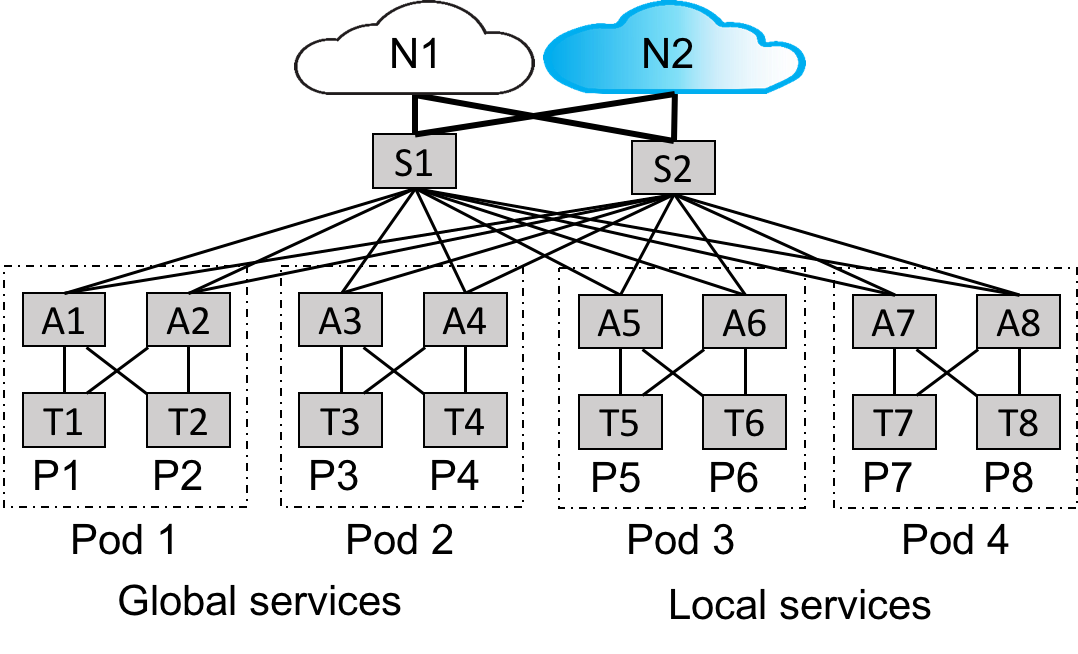
\includegraphics[width=2.5in]{figures/example}
  \caption{An example data center network.}
  \label{fig:example}
  \vspace{-1em}
\end{figure}

\begin{figure}[t!]
  \centering
  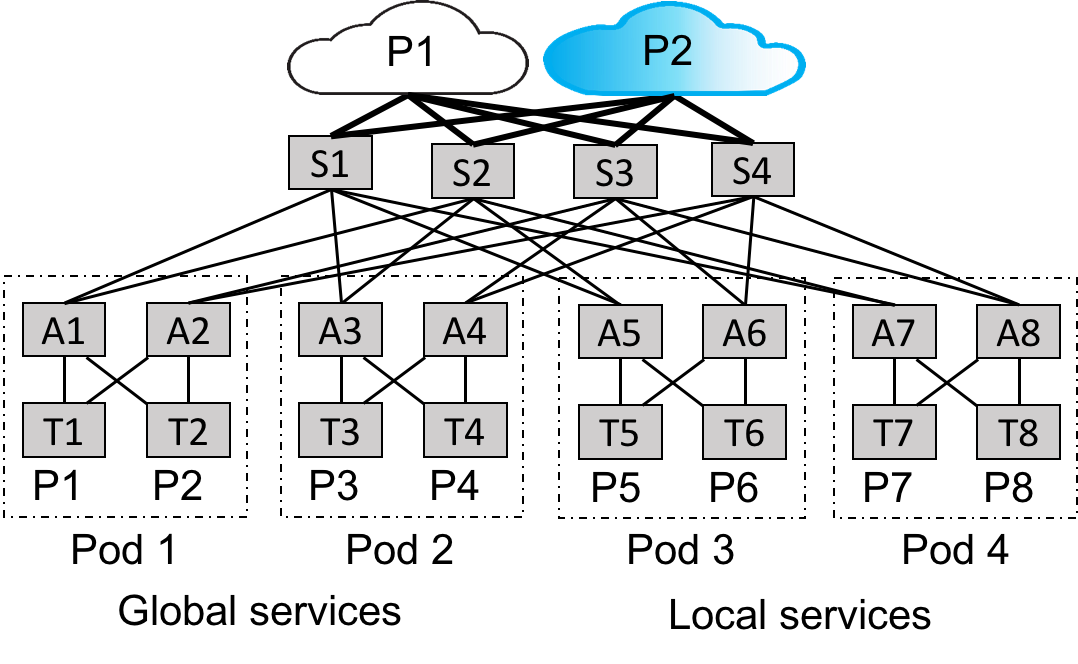
\includegraphics[width=2.5in]{figures/example2}
  \caption{A modified version of the example in Figure~\ref{fig:example}.}
  \label{fig:example2}
  \vspace{-1em}
\end{figure}

We demonstrate the difficulty of configuring networks using the example data center network in Figure~\ref{fig:example}. The boxes denote routers. Using terminology for fat tree networks~\cite{fattree}, S[1--2] denote spine routers, A[1--8] denote aggregation routers, and T[1--8] denote top-of-rack (ToR) routers. The spine routers are connected to the
rest of the Internet through neighbors N[1--2]. The aggregation routers
bridge the spine to the ToR routers. The ToR routers attach to a set of servers (``a rack'') that host services with address prefixes P[1--8].

%% We assume that each router is running an instance of the \emph{Border Gateway Protocol} (BGP),
%% as is common in large data centers. In this protocol, adjacent routers use BGP to exchange messages
%% with one another concerning the availability of routes to destinations.  A BGP \emph{configuration}
%% (one for each router) dictates which offered routes a router will select and how to propagate chosen routes to its
%% neighbours.\footnote{If this submission is accepted and more space is available in the final version,
%% we will give a detailed explanation of BGP for the PLDI audience.  Henceforth, we assume knowledge of basic BGP
%% mechanics.}

%Assume that all nodes are running the border gateway protocol (BGP), as is common in large data centers~\cite{x}. \todo{more detail on BGP?}

The intended policy for this network is:
$(1)$ complete internal connectivity, \IE, all routers should be able to talk to each other;
$(2)$ services in Pods[1--2] should be globally accessible;
$(3)$ prefixes for global service should be aggregated into a covering prefix PG when announced outside;
$(4)$ services in Pods[3--4] should not be externally accessible;
$(5)$ paths should be valley-free, \IE, never go down then back up.
$(6)$ prefer neighbor N1 over N2, \IE, when both neighbors announce a prefix, send traffic through N1;
$(7)$ datacenter routers should not transit traffic between N1 and N2; and
$(8)$ no loss in connectivity after any single-link failure.

To correctly configure this policy, network operators must generate configurations for each router. This implies ensuring, for instance, that all router interfaces are assigned correct addresses; all routing adjacencies are correctly configured (\EG, T1's configuration includes A1 as neighbor and vice-versa); all routers announce their own addresses (so that they can be reached from other routers) and the ToRs announce the correct prefixes for their services; all routers  forward the prefix announcements that they should to each neighbor and not forward those that they should not (\EG, the spines should forward prefixes for local services to internal neighbors but not external neighbors); and the spines announce externally only the aggregate global prefix. Such configuration tasks are highly complex~\cite{juniper-study,bgpmon,batfish,propane}.

To simplify network configuration, the operations community is adopting a template-based approach~\cite{hatch,thwack}. Instead of authoring a configuration file per router, operators author one configuration template per role.
%
A {\em role} refers to specific functionality and is played by one or more routers.\footnote{If a role is played by devices from multiple vendors, there is one template per role-vendor combination because templates use vendor-specific configuration languages.}
%
The network in Figure~\ref{fig:example} might have five roles: spine, global aggregator, global ToR, local aggregator, and local ToR.
%
Templates have parameters for various aspects of the configuration (\EG, interface addresses, neighbor list) and are compiled to device configurations by instantiating the parameters using a database of network information.

%Templates provide two key advantages. First, they help eliminate a class of configuration errors that stem from typos and inconsistencies, e.g., using the wrong address for a router, having inconsistent addresses for the two ends of a link, and failing to configure one side of a routing adjacency.  Second, templates have the potential for re-use when the topology changes while maintaining its basic structure (e.g., adding a new pod to the data center) or multiple networks with similar structures need to be instantiated (e.g., in an organization that runs multiple data centers).

%While templates help avoid a class of configuration errors (e.g., inconsistent routing adjacencies), they provide no guarantees
Templates that work for one topology may not work for seemingly-inconsequential variations.  
%Unfotunately, currently, there is no way to predict which variations will behave correctly for a given set of templates.
Worse, when operators discover their old templates no longer work, changing a template will
cause a change to all devices that use that template---an unacceptable disruption in many cases.  When that happens, operators may abandon templates entirely and revert to hand-crafting configurations, using local patches to accommodate the change.
Such patches reintroduce the complexity and errors that templates were meant to prevent.

%they are difficult to author. Operators must manually decompose complex, network-wide routing policy into role templates such that the collective behavior of the configurations generated from them will correctly implement the policy, both when failures occur and as the network evolves.

%This task is error-prone, and no tools exist today for template verification; in fact, such tools would be difficult to build as templates have no semantics, of policies or topologies they were intended to work for, independent of the configurations they produce. Today, operators test (not verify) templates by simulating their generated configurations over the current or known future topologies.

%As a result, the types of configuration design errors pointed in prior work~\cite{propane} can occur in template design as well. For instance, to keep local prefixes internal the engineer may implement announcement forwarding on spines based on the identity of the neighbor, \IE, do not announce externally anything heard from local aggregators. This implementation is appealing because it does not require changes to spine configurations when ToR prefixes change. But it works correctly only when there are no failures; local prefixes can leak externally when failures disconnect a spine from both aggregators in a local pod. Specifically, when S1 is disconnected from A5 and A6, it may hear about P5 and P6 from A3 and A4 (via A[5--6]->S2->A[3--4]), and it will then announce those prefixes outside (since they no not come from a local aggregator), leading to a policy violation. A possible correct implementation here would be for each spine to block messages headed to external peers from local aggregators {\em and} to reject announcements that have traversed the other spine (\IE, to disallow "valleys," or up-down-up paths).

%Lacking correctness guarantees, engineers use simulations to analyze if templates are correct under a range of failure cases (e.g., combinations of two-link failures), but such analysis is highly expensive for large networks and still does not provide strong guarantees beyond the tested cases.

%The second limitation of today's template systems is that, like concrete synthesis tools, they do not support network evolution. One might hope that important network properties such as connectivity and fault tolerance persist when networks evolve in ways consistent with existing roles and templates.  However, existing template systems provide no guarantees that seemingly-minor variations of a given topology have similar properties.
%In theory, templates do not have to be redesigned when the network evolves while keeping its basic structure of roles and their inter-connectivity. In practice, however, it is not guaranteed that templates that work for a given topology also work for seemingly-minor variations of the topology.

%Such simulations provide some assurance that the templates work correctly for the simulated topologies but little assurance for other topologies that may arise after the network evolves. 

%Templates that work for one topology may not work for seemingly-inconsequential variations.  
%Unfotunately, currently, there is no way to predict which variations will behave correctly for a given set of templates.
%Worse, when operators discover their old templates no longer work, changing a template will
%cause a change to all devices that use that template---an unacceptable disruption in many cases.  When that happens, operators may abandon templates entirely and revert to hand-crafting configurations, using local patches to accommodate the change.
%Such patches reintroduce the complexity and errors that templates were meant to prevent.

%% For some changes, they may discover that their old templates will not work anymore. ~\dpw{Note: This is going to be true for Methane too.} ~\ratul{Not really; our abstract topologies encode all possible future topologies} ~\dpw{Our abstract topologies precisely define a set of topologies for which our
%% This discovery is highly problematic because changing a template may cause a configuration change of all the devices that use that template---an unacceptable disruption in many cases.  When that happens, network operators may abandon templates entirely and revert to hand-crafting configurations, using local patches to accommodate the topological change.
%% Such patches reintroduce the complexity and errors that templates were meant to prevent.

Consider the network in Figure~\ref{fig:example2}, which is similar to Figure~\ref{fig:example}; it has the same five roles, connected in a similar hierarchy. One might think that the same templates (with different database entries) can be used for both topologies. However, because the templates are configured to disallow ``valley" paths, which go down, and then up, these templates will work perfectly for Figure~\ref{fig:example} but silently violate the fault tolerance requirement ($(8)$) when used for Figure~\ref{fig:example2}.  Specifically, in Figure~\ref{fig:example2}, an aggregation-induced blackhole (\S\ref{sec:background}) will occur when the link S1--A1 fails; after this failure, S1 has no valley-free path to P[1--2] even though it will continue to get traffic for these prefixes as it announces the covering prefix PG (because it gets routes for P[3--4]). In contrast, in Figure~\ref{fig:example}, no such blackhole will occur after a single link failure because spine routers have two links to each pod.

%% Thus, today, operators test templates for each topology change. For some changes, they may discover that their old templates will not work anymore. ~\dpw{Note: This is going to be true for Methane too.} ~\ratul{Not really; our abstract topologies encode all possible future topologies} ~\dpw{Our abstract topologies precisely define a set of topologies for which our
%% This discovery is highly problematic because changing a template may cause a configuration change of all the devices that use that template---an unacceptable disruption in many cases.  When that happens, network operators may abandon templates entirely and revert to hand-crafting configurations, using local patches to accommodate the topological change.
%% Such patches reintroduce the complexity and errors that templates were meant to prevent.


%\para{Configuration synthesis with concrete topologies}
%Many recent systems generate router configurations using high-level policy statements~\cite{narain:lisa05,narain+:configassure,dadc,propane} and the network's concrete topology.
%%These systems eliminate entire classes of configuration errors by construction, and, in the case of
%%Propane~\cite{propane}, guarantee that high-level policy is implemented correctly, even in the presence of
%%arbitrary combinations of failures.
%They are able to provide strong guarantees on configuration correctness but
%our conversations with operators at two major cloud providers reveal that they have two limitations that discourage adoption.  The first is abstraction mismatch. Operators of large networks think of the network, and develop management tools, using \emph{roles}, and not individual devices. They are naturally reluctant to use a system that does not
%understand roles as a first-order abstraction. If they want to debug, analyze or
%understand system output, they will have to consider
%\emph{hundreds} of independent device configurations instead of just
%\emph{a handful} of role configurations. Unfortunately, even if two devices play the same role,
%there is no guarantee a concrete synthesis system will generate (syntactically) similar configurations.
%
%%A second limitation is the inability to support network evolution. Networks evolve all the time as nodes and links are added or removed and the addresses of services are changed. A system that supports evolution would ensure that
%%small changes in topology require small, local changes in network configurations as opposed to pervasive
%%changes across many devices.  Engineers want to minimize changes to device configurations because each change runs the risk of poor, transient behavior due to poor router software or routing protocol dynamics~\cite{ratulbgpmisconfigs}.
%%These networks must be highly
%%available; it isn't plausible to bring down an entire data center network, or large portions of it, to make
%%incremental changes.
%
%Second, these systems become even more brittle in the face of network evolution.
%Any change in network topology requires re-execution of a
%concrete synthesis engine, from scratch,
%on the changed topology.  The result may be
%a completely different set of configurations.  Even if such configurations are
%largely semantically similar to existing configurations, they may be syntactically different and cause considerable network disruption when updates are pushed to routers.

%For instance, suppose an operator wants to modify the prefix of local ToR T8 in Figure~\ref{fig:example}. To accommodate the modification, Propane, a concrete synthesis tool, will, at a minimum, not only change T8's configuration but also those of the two spines because it uses prefix lists at spines to ensure that local prefixes are not advertised externally.  As we show later, there is a way to design the configurations of this network to avoid spine configuration changes while accommodating ToR prefix (and other) modifications.  Our new abstraction-based synthesis framework synthesizes evolution-friendly roles automatically.

%nof the new spine configurations outputted by Propane will not only enable the interfaces that connect to the new aggregators but will also have to update the prefix list filters. A system that supports incremental growth should need only interface configuration changes (not filter changes). It can configure all local ToRs, including the new ones, to attach a tag to their announcements and filter external announcements at the spines based on this tag. Engineers prefer fewer configuration changes because each change runs the risks of poor transient behavior (which synthesis tools do not reason about).


%For instance, suppose the engineers want to add another pod with local services to the network in Figure~\ref{fig:example}. In this network, Propane, a concrete synthesis tool, uses prefix lists at spines to ensure that local prefixes are not advertised externally. To accommodate the expansion, the new spine configurations outputted by Propane will not only enable the interfaces that connect to the new aggregators but will also have to update the prefix list filters. A system that supports incremental growth should need only interface configuration changes (not filter changes). It can configure all local ToRs, including the new ones, to attach a tag to their announcements and filter external announcements at the spines based on this tag. Engineers prefer fewer configuration changes because each change runs the risks of poor transient behavior (which synthesis tools do not reason about).




%As an aside, a possible template implementation that works correctly for both networks is: allow valley paths and use an explicit list of local prefixes at spines to decide which announcements should not be forwarded externally.

%\begin{figure}
%\begin{tabular}{|p{0.6in}|p{0.6in}p{0.7in}p{0.6in}|}
%\hline
%& Abstract Roles & Correctness Guarantees & Evolution Support  \\ \hline
%Concrete Synthesis & \xmark & \cmark & \xmark \\ \hline
%Template Systems & \cmark & \xmark & \xmark \\ \hline
%\sysname & \cmark & \cmark & \cmark \\  \hline
%\end{tabular}
%\caption{Comparing configuration techniques.}
%\label{fig:marketing}
%\end{figure}

%\subsection{\sysnamesec}
%
%As Table~\ref{fig:marketing} shows, \sysname addresses the limitations of both concrete synthesis and current template systems. It operates at the right level of abstraction for network operators, provides strong guarantees about compiled configurations, supports verification of important correctness properties, and supports network evolution.

%=====================================================
%
%
%  **Methane Overview**
%
%
%=====================================================

\section{Methane overview}
\label{sec:overview}

In this section we give an overview of \sysname, a system for generating provably-correct templates from the network's policy and an {\em abstract} topology that describes device roles and connectivity invariants.
%As inputs, it takes a global, network-wide policy (as opposed to a per-device or even per-role policy) and an {\em abstract} topology that describes device roles and connectivity invariants.  It outputs a template for each role, from which per-device configurations can be generated by instantiating parameters with values drawn from the network topology.
%It guarantees that:
%(1) the configurations generated from its templates correctly implement the network's policy for {\em any} concrete topology that matches the abstract topology; and (2) if nodes or edges are added or removed in a way compatible
%with the abstract topology, only configurations of devices adjacent to the change ever need to be updated.
%
%This section introduces \sysname using the examples in \S\ref{sec:motivation}.
%, and the following sections detail template generation and formally define the correctness guarantees.
%
When \sysname generates templates, it guarantees that the forwarding behavior of the network will be correct for any instantiation of the templates on a concrete network that repects the abstraction. 
%Furthermore, \sysname will generate configurations in such a way that, if an operator expands their network in a way compatible with the abstraction, then only configurations of devices adjacent to the change ever need to be updated.


\subsection{Inputs}

\sysname takes as input the network's abstract topology and its policy. The policy has two components: the routing policy describes how traffic should flow, and the fault-tolerance policy describes how many simultaneous failures the network can withstand without loosing connectivity.

\para{Abstract topology}
Abstract topologies in \sysname define structural and role-based invariants that capture a collection of concrete networks. These invariants are encoded in the form of a graph homomorphism annotated with logical constraints about node and edge multiplicities and connectivity.
%
We designed these abstractions to be able to precisely capture most real network topologies, while being amenable to the fault tolerance analysis and configuration synthesis that is done by our compiler.

%Ideally, we would like to find a suitable topology abstraction that can describe both of the datacenters from figures~\ref{fig:example} and~\ref{fig:example2} as well as any reasonable generalization of these datacenters. \sysname provides several abstraction mechanisms to achieve this goal.

We introduce our topology abstractions using the networks from \S\ref{sec:motivation}. Topology abstractions consist of several components.
The first is a role-based abstraction that allows an operator to map routers in the concrete network to roles in the abstract network. Figure~\ref{fig:example3} shows an example of an abstraction for both datacenter networks from \S\ref{sec:motivation}. In the example, the concrete networks are abstracted into a new topology with 5 different roles: local ToR (TL), global ToR (TG), local aggregator (AL), global aggregator (AG), and spine (S).

More specifically, a network topology is a graph $G$ = ($V, E$), which consists of a set of vertices $V$ and a set of directed edges $E \colon V \times V$. A role-based abstraction is a graph homomorphism from $G$ to an abstract graph $G^A$ = ($V^A$,$E^A$). A graph homorphism $f : G \rightarrow G^A$ maps each node in the concrete graph to a node in the abstract graph such that, whenever $(u,v) \in E$, then $(f(u),f(v)) \in E^A$.


\begin{figure}[t!]
  \centering
  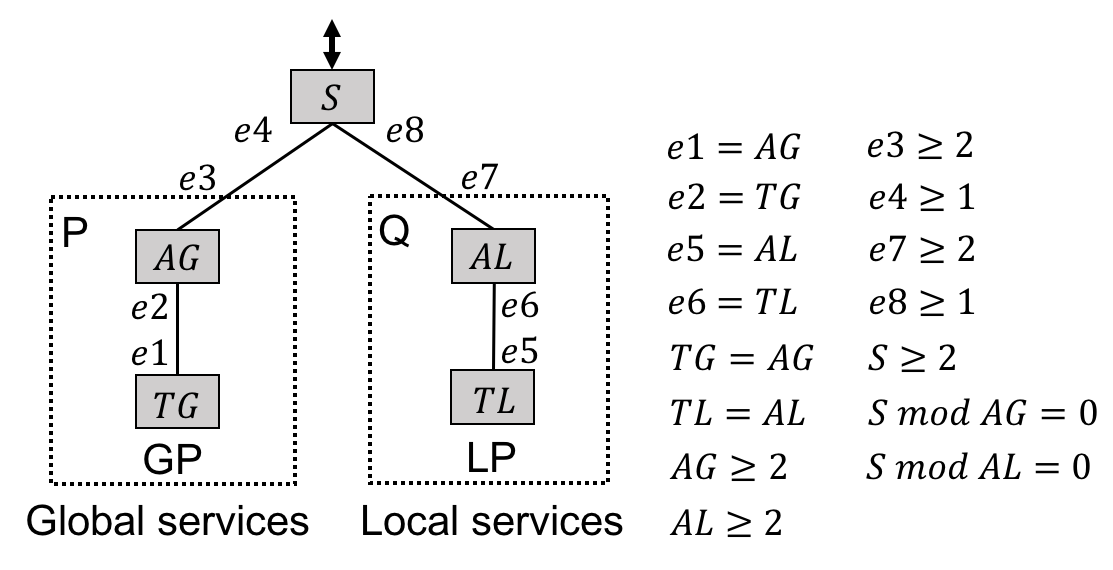
\includegraphics[width=\columnwidth]{figures/example3}
  \caption{An abstraction for the datacenters in Figure~\ref{fig:example}.}
  \label{fig:example3}
  \vspace{-1em}
\end{figure}

The role-based abstraction therefore overapproximates the connectivity of the underlying concrete graphs. On its own, this abstraction loses a lot of information about the underlying structure of the concrete network, making it difficult to reason precisely about fault-tolerance.
%which would hinder a useful analysis of its fault-tolerance.
For example, with this abstraction any spine router in a concrete network may or may not be connected to any aggregator router.
%
In order to refine the abstraction to capture more precisely the kinds of concrete networks of interest,
we introduce several additional concepts. The first is the idea of a topology hierarchy captured by P and Q, which say that nodes in the tor and aggregator roles are grouped into a number of smaller pods.
The second is a notion of node and edge \emph{multiplicities}. Each edge (and node) is labelled
with a symbolic variable (\EG, $e1, e2, \ldots$) that denotes a constraint on the number of edges (and nodes) that may appear in any given concrete network. Operators can capture concrete network invariants by adding constraints on the symbolic variables using logical formula.

For example, in Figure~\ref{fig:example3}, the first two constraints: $e1 = AG$ and $e2 = TG$ say that, within any pod P, the number of outgoing edges from a node in the $TG$ role to a node in the $AG$ role is equal to the number of nodes in the $AG$ role. Similarly, the number of outgoing edges from a node in the $AG$ role to a node in the $TG$ role is equal to the number of nodes in the $TG$ role. These constraints capture the fact that, within any given pod, the global aggregators and ToRs are in a full mesh. Furthermore, the constraints $AG = AL$ and $AG \leq S$ ensure that, within pods P and Q, the $AG$ and $TG$ roles have the same number of routers, which is less than the number of routers in the spine role $S$.
%
The constraint $e3 \geq 2$ says that, in each pod, each aggregator node has at least 2 outgoing edges to nodes in the spine role. Symmetrically, the constraint $e4 \geq 1$ says that, for each pod P, each node in the spine role has at least one outgoing edge to a node in the $AG$ role. Similar constraints appear for the local aggregator role. The constraint $2 \leq S \leq 4$ makes explicit the possibility for growth, for example by growing the network from that of Figure~\ref{fig:example} to that of Figure~\ref{fig:example2}. In general, we need not bound the number of spine routers to admit more concrete topologies, potentially at the expense of analysis precision. Finally, we include the constraints $(S \mod AG) = 0$, and $(S \mod AL) = 0$ simply to show that constraints do not have to be inequalities. In general operators can write constraints using logical formula from any theory supported by modern SMT solvers.

A final type of abstraction is the $mincut(1)$ constraint between the spine role S and N[1--2]. The mincut constraint says that any node in the spine role has at least one path to any node in the neighbor N1 (and N2) role. Annotations of this form are often useful for a "one big switch" \ryan{cite} type of abstraction where part of a complex network is abstracted into a single node. For example, to model an ISP backbone network the operator might abstract the network into separate geographic regions with two abstract roles per region -- one role for the border routers of the network, and another role for the core of the network. Mincut annotations could be used to describe the fault tolerance both within region cores as well as across regions.

%All the guarantees provided by \sysname hold for any instantiation of the abstract network. This means that operators can safely expand their network in the future so long as the new network also satisfies these logical constraints.

%Although the concrete \sysname policy can help prevent a number of configuration errors,
%the policy is intricately linked to the actual structure of the concrete network.
%For example, each prefix in the routing constraint is enumerated with its concrete destination
%location, and the definition of the valleyfree constraint depends on the actual routers that
%comprise each tier of the datacenter.
%
%This is unfortunate since any expansion of our datacenter network will require a corresponding
%change to the policy. Furthermore, there is no guarantee that a safe policy can be found
%for the expanded network, and even if one can be found, it may require changes to every
%configuration in the network -- a huge barrier to adoption in practice.

%Abstract \sysname solves this problem in two ways. First, it allows operators to abstract
%the network into a role-based topology and write a routing specification over this abstraction instead.
%Second, it introduces prefix template variables into the language to allow writing policies that are
%parameterized over prefix destination.

\para{Routing policy} Routing policies in \sysname consist of an ordered sequence of both a predicate matching a class of traffic and a list of ranked constraints on the paths that the traffic matching the predicate should prefer to take through the network. We borrow syntax from Propane~\cite{propane} but, instead of concrete prefixes and nodes, \sysname specifications can use abstract prefixes and nodes.

Let us see how to configure each of the datacenter networks from \S\ref{sec:motivation} by writing a \sysname routing policy over the abstract topology. We can capture the basic routing behavior, constraints (1, 2, 6), for the datacenters with the following policy:
%
\begin{code}
\Define Routing =
    \$GP  \Path \End(TG)
    \$LP  \Path \End(TL)
    \True \Path \End(\Out) & \Exit(N1 \Prefer N2)
\end{code}
\noindent%

The first line introduces a prefix \emph{template} variable. It says that traffic for each global prefix associated with the template variable $\CD{\$GP}$ has the constraint that it should follow a path that ends at its corresponding destination router contained in the $\CD{TG}$ role. The second line does the same for all local prefixes.
%
The final rule matches all other IP prefix destinations and allows traffic to follow a path that leaves the datacenter, ending up at some outside location, through either of its peers $\CD{N1}$ or $\CD{N2}$ with a preference for leaving through $\CD{N1}$ over $\CD{N2}$. The $\CD{\Prefer}$~symbol indicates that traffic should satisfy the constraint on the left whenever possible (\IE, a path exists in the network), and only resort to the backup (right) when this is not possible due to network failures.%

Next we can capture constraint (4) that traffic for local prefixes must stay local to the datacenter:
%
\begin{code}
\Define Local =
    \$LP \Path \Always(\In)
\end{code}
\noindent%
%
The Local constraint applies to any traffic destined for a local prefix described by the $\CD{\$LP}$ prefix template variable and adds the constraint that the traffic must follow a path that matches an internal location (\IE, a router inside the datacenter) at each hop of the path.
%
The constraint to prevent "valleys" (5) is implemented as:
%
\begin{code}
\Define NoValley =
    \True \Path \Novalley(\{TG,TL\},\{AG,AL\},\{S\})
\end{code}
\noindent%
%
This policy applies to all traffic and prevents valley paths by adding the $\Novalley$ constraint with arguments corresponding to each datacenter level.
%
Constraint (7) to prevent transit traffic between neighbors is expressed in \sysname as:
%
\begin{code}
\Define Peer = \{N1,N2\}
\Define NoTransit =
    \True \Path !(\Enter(Peer) & \Exit(Peer))
\end{code}
\noindent%
%
We define a $\CD{Peer}$ to be either $\CD{N1}$ or $\CD{N2}$ and disallow paths where traffic both enters the datacenter through a peer and exits through a peer. Finally, we can combine these constraints together as follows:

\begin{code}
Routing & Local & NoTransit & 
NoValley & \Agg(PG, \In -> \Out)
\end{code}
\noindent%

This instructs \sysname to find BGP router configurations that satisfy the conjunction of all the constraints. It also declares an additional constraint that we want to perform prefix summarization (as PG) for global prefixes at the border of the datacenter (\IE, along any edge starting inside our datacenter and ending at a peer outside the datacenter).

\para{Fault-tolerance policy} This policy specifies how many link failures the network should be able to withstand before connectivity loss for traffic occurs. Operators can  specify different tolerance levels for different pairs of abstract nodes. For instance, they may say that ToR to spine connectivity should be robust to 2 failures, \IE, no ToR-spine pair should lose connectivity as long as the number of simultaneous link failures is 2 or fewer; and ToR-to-ToR connectivity should be be robust to 1 failure.

\subsection{Compilation}

%\sysname builds on the Propane network configuration tool, by supporting both synthesis for and reasoning over parameterized classes of topologies and their interactions with user-specified routing policy.

%Although \sysname can ensure correct forwarding behavior independent of the exact concrete topology or failure scenario, it is often useful to be able to ask "what if" questions about other network properties. For example, an operator may require a certain level fault tolerance between between different collections of routers. Such analysis depends, not only on the network topology, but also on the underlying routing policy, both of which \sysname has access to.
The \sysname compiler generates templates from the inputs above in three phases. First, it combines the abstract topology and routing policy into a {\em product graph} that compactly captures the flow of routing information over the topology in a policy-compliant manner. The algorithm for this phase builds on the Propane compiler, which was designed for concrete topologies and policy; we show that it can be extended to abstract inputs and that the extensions are correct.

Second, \sysname checks if the fault-tolerance policy can be met by considering the joint impact of the abstract topology and routing policy. Joint analysis is needed, because connectivity for traffic will suffer even when functional paths exists in the topology if those paths are not allowed by routing policy. It implies that we cannot use standard graph theoretic algorithms.

Instead, we develop a sound analysis based on computing the minimum number of disjoint policy-compliant paths between pairs of nodes over abstract topologies. If this number for a pair of nodes is less than the desired fault-tolerance level, \sysname declares that the policy cannot be met.

Suppose we want to compute the number of of disjoint paths between any global ToR and spine router in Figure~\ref{fig:example3} for any concrete topology after applying the routing policy.
%This can be used as a lightweight verification tool to detect certain classes of configuration bugs. For example, since the network is performing prefix summarization at the border of the datacenter, we might introduce a black hole after enough failures occur to disconnect a tor from a spine router.
For each abstract role in the network, we learn invariants about the number of disjoint paths to routers in that role. These invariants contain a sequence of labels followed by a pair of numbers $(i,j)$. For example, the analysis would start with a fact of the form: $S_P S_{TG} (1,1)$. This means that, there is some group of nodes of size 1 in the TG role in some pod P such that any initial node in the TG role has 1 disjoint path to it (and all such paths are edge-disjoint). Since we know that the each node in the TG role is in a full mesh with nodes in the AG role within any given pod, we might infer a fact for AG of the form: $S_P A_{AG}(e1,1)$. This says that any group of nodes of size e1 in the AG role is reachable with at least 1 edge-disjoint path to each such node from any initial node in the TG role.
%
After one more inference the analysis will learn a fact of the form $A_{S}(1,1)$, which means that any single spine node is reachable via a single disjoint path from any initial global ToR node 
In fact, due the the valley-free routing constraint, a single path is the most information we can infer, since this is exactly the worst-case fault-tolerance for the concrete network from Figure~\ref{fig:example2}.

If \sysname finds that the fault-tolerance policy can be met, it generates templates for the abstract topology, which can be instantiated into BGP configurations based on the concrete topology. During concretization, we confirm that the concrete topology adheres to the abstract topology.

%
%The constraint prevents traffic from over taking a path that traverses
%either [Agg->Tor->Agg] or [Spn->Agg->Spn]. The final policy remains the same as before,
%by combining each of these policies together.
%
%


%=====================================================
%
%
%  **Language and Product Graph**
%
%
%=====================================================

\section{Product Graph Generation}
\label{sec:language}

%Configuration synthesis for network configurations is challenging for a number of reasons. First, although \sysname polices specify network-wide routing behavior, actual configurations are per-device and run distributed algorithms to compute routes. Thus the compiler must ensure that the result of the distributed interaction of devices correctly implements the policy including when failures occur. Second, \sysname must find configurations that work for any valid concrete network topology matching the user-specified abstraction. Finally, \sysname must ensure that the resulting configurations can be evolved incrementally so that local changes to the topology ensure that only local changes to configurations are required to ensure global routing correctness.

%In this section, we formalize the \sysname language and describe how \sysname translates policies to a graph-based intermediate representation.

%\subsection{Methane Language}

\begin{figure}[t]\small
  \begin{minipage}[t]{\linewidth}
  \vspace*{-1\baselineskip}
  %
  \[ \begin{array}{rclr}
     pol     &::=& p_1, \dots, p_n & \textit{policy} \\
     p       &::=& t \hspace{.3em} \Path \hspace{.3em} r_1 \Prefer \dots \Prefer r_m \BNFALT a & \textit{path preferences}  \\
     t       &::=& \$x \BNFALT d.d.d.d/[d..d] \hspace{1.5em} & \textit{predicate} \\
     a      &::=& agg(t, r_1 \rightarrow r_2) & \textit{aggregation} \\
     r       &::=& l \BNFALT \emptyset \BNFALT \In \BNFALT \Out \BNFALT r_1 \cup r_2 \BNFALT & \textit{regular path} \\
             &   & r_1 \cap r_2 \BNFALT r_1 \cdot r_2 \BNFALT \NOT r \BNFALT r^* \\
%         &\BNFALT& \emptyset & \textit{empty set} \\
%         &\BNFALT& \In & \textit{internal loc} \\
%         &\BNFALT& \Out & \textit{external loc} \\
%         &\BNFALT& r_1 \cup r_2 & \textit{union} \\
%         &\BNFALT& r_1 \cap r_2 & \textit{intersection} \\
%         &\BNFALT& r_1 \cdot r_2 & \textit{concatenation} \\
%         &\BNFALT& \NOT r & \textit{path negation} \\
%         &\BNFALT& r^* & \textit{iteration} \\
  \end{array} \]%

  \end{minipage}
  \vspace{-.3em}
  \caption{\sysname core syntax.}
  \label{fig:syntax}
  %\vspace{-1em}
\end{figure}%

The syntax introduced in \S\ref{sec:overview} is just syntactic sugar for a core language based on regular expressions. Figure~\ref{fig:syntax} shows the core \sysname syntax.
%
A policy has one or more constraints, each of which is either an aggregation constraint or a path constraint. Path constraints consists of a test on a prefix destination and a list of regular expressions describing preferred network paths. Regular paths are defined over network locations, where each location is either a router inside the operator's network, or an external neighbor connected to the operator's network. Values \In~ and \Out, will match any internal and external location respectively. There are two types of predicates: a test for a concrete prefix $d.d.d.d/[d..d]$ matches a range of IP prefixes (\EG, 10.0.1.0/[24..32]) where metavariable $d$ represents an integer.

Converting from the high-level syntax from \S\ref{sec:overview} to the core syntax is straightforward. The predicate $\True$ becomes the prefix range $0.0.0.0/[0..32]$.
%
Each constraint desugars to a regular expression. For example, the constraint $\Always\CD{(\In)}$ becomes $\In^*$ and the constraint $\CD{\End(T0)}$ becomes $\mathtt{\Sigma}^* \cdot \CD{T0}$.
%
Preferences are lifted to the top level of the regular expression when their use is unambiguous, and separate sets of constraints are joined prefix-by-prefix by taking the set intersection of their constraints.

%For example, the combining the Routing and Local constraints in the data center policy from \S\ref{sec:overview} would result in the following \sysname policy:
%
%\begin{code}
%\$PG  \Path \End(TG),
%\$PL  \Path \End(TL) \ensuremath{\cap} \Always(\In),
%\True \Path \Exit(Peer1) \Prefer \Exit(Peer2)
%\end{code}
%\noindent%
%

A key step for \sysname to generate device configurations is to build a data structure amenable to joint analysis of both the topology and routing policy. Intutively, \sysname captures both topology and routing constraints by ``intersecting" the finite automata associated with the policy regular expressions with the graph structure of the topology into a data structure called the Product Graph~\cite{propane}.

The Product Graph compactly encodes all paths protocol messages should be passed along through the network in order to guarantee the devices find policy-compliant paths dynamically.
%
%Although \sysname policies describe the routes that traffic should take through the network, network protocols (including BGP) typically disseminate router information in the opposite direction. For example, a router Y will tell its neighbor X that it has a route to the destination meaning that X can send traffic through Y. For this reason, we start by compiling
%
Because \sysname policies can have a separate routing policy for each predicate matching traffic, we construct one such Product Graph for each predicate.


For each regular path constraint $r_i$ from $r_1 ~\Prefer~ .. ~\Prefer~ r_k$, we construct a DFA for the reverse of $r_i$. A DFA for $r_i$ is defined as a tuple ($\Sigma, Q_i, F_i, q_{0_i}, \sigma_i$). The alphabet $\Sigma$ is the set of topology locations, $Q_i$ is the set of states for automaton i, $F_i$ is the set of final states, $q_{0_i}$ is the initial state, and $\sigma_i \colon Q_i \times \Sigma \rightarrow Q_i$ is the state transition function.
%
The Product Graph is a tuple ($G'$, $start$, $P$) where $G' = (V',E')$ is a new graph with
vertices $V' \colon V \times Q_1 \times \dots \times Q_j$,
edges $E' \colon V' \times V'$,
a unique starting vertex $start$,
and a preference function $P \colon V' \rightarrow 2^{\set{1, \dots, j}}$, mapping nodes in the product graph to a set of path ranks.

The Product Graph is constructed by adding an edge from state $m = (l_m, q_{m_1}, \dots, q_{m_k})$ to $n = (l_n, q_{n_1}, \dots, q_{n_k})$ whenever $\sigma_i(q_{m_i}, l_n) = q_{n_i}$ for each $i$ and $(l_m,l_n) \in E$ is a valid topology link.
%
We add edges from the start node to any $m = (l, q_{m_1}, \dots, q_{m_k})$ when $\sigma_i(q_{0_i}, l) = q_{m_i}$ for each $i$.
%
The preference function $P(m)$ denotes the rank of paths through the Product Graph ending at node $m$ and is defined as $P(m) = \set{i~\vert~q_{m_i} \in F_i}$.
%
Finally, we write $\tilde{m} = l$ to extract the topology location from a product graph node, when $m = (l, q_{m_1}, \dots, q_{m_k}) \in V'$.

Figure~\ref{fig:example-compilation} shows an example of a Product Graph for the policy that applies to all external traffic from the datacenter example in \S\ref{sec:overview} ($\True ~\Path~ \CD{\Exit(N1 \Prefer~N2)}$).
%
%\begin{code}
%\True \Path \Exit(\sf{Peer1}) \Prefer \Exit(\sf{Peer2})
%\end{code}
%\noindent%
%
The first automaton represents the more preferred constraint $\CD{\Exit(N1)}$ and the second automaton represents the less preferred constraint $\CD{\Exit(N2)}$. The Product Graph is shown for both an instance of a simple concrete network matching the abstraction from \S\ref{sec:overview} as well as for the abstract topology.

Paths through the Product Graph represent paths through the topology that protocol messages may use to ensure policy-compliant. For example, in the concrete Product Graph, all messages from N1 are not blocked at each spine router. Paths for a destination learned through N1 will end in an accepting state for the first automaton (\EG, node (T1,1,0)). Similarly, paths for a destination learned through N2 will end in an accepting state for the second automaton. 

One interesting observation is that the Product Graph for both the concrete and abstract networks share a similar structure. This leads us to the following observation:

\begin{defn}
If we have a graph homomorphism $f : G \rightarrow G^A$, concrete product graph $PG = (G',\mathit{start},P)$ and abstract product graph $PG^A = (G'^A, \mathit{start}^A, P^A)$, then we can construct a new homomorphism $f_{pg} : G' \rightarrow G'^A$:
\[ \begin{array}{rcl}
  f_{pg}( \mathit{start} ) & = & \mathit{start}^A  \\
  f_{pg}( (l,q_1,\ldots,q_n) ) & = & (f(l),q_1,\ldots,q_n) \\
\end{array} \]
\end{defn}

\newcommand{\state}[4]{\node[state,#3](#1)[#4]{#2};}
\newcommand{\transition}[4]{\path[->] (#1) edge [#4] node {#3} (#2);}

\begin{figure*}[t!]
  \begin{minipage}[t]{.4\linewidth}
  \hdr{Policy Automata}{}
  \vspace{1em}
    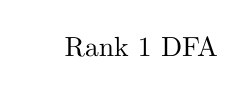
\begin{tikzpicture}[>=stealth',shorten >=1pt,auto,node distance=2cm,minimum size=.5cm]
      \state{0}{$0$}{              }{}
      \state{1}{$1$}{right of=0}{accepting}
      \transition{0}{0}{out}{loop above}
      \transition{0}{1}{Peer1}{}
      \transition{1}{1}{in}{loop above}
      \node at (1,-1){Rank 1 DFA};
    \end{tikzpicture}
    ~~~~~
    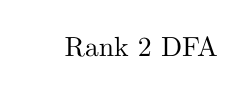
\begin{tikzpicture}[>=stealth',shorten >=1pt,auto,node distance=2cm,minimum size=.5cm]
      \state{0}{$0$}{              }{}
      \state{1}{$1$}{right of=0}{accepting}
      \transition{0}{0}{out}{loop above}
      \transition{0}{1}{Peer2}{}
      \transition{1}{1}{in}{loop above}
      \node at (1,-1){Rank 2 DFA};
    \end{tikzpicture}%
  \end{minipage}
  %
  ~~~~~~
  %
  \begin{minipage}[t]{.3\linewidth}
    \hdr{Concrete Topology}{}
    \vspace{1em}
    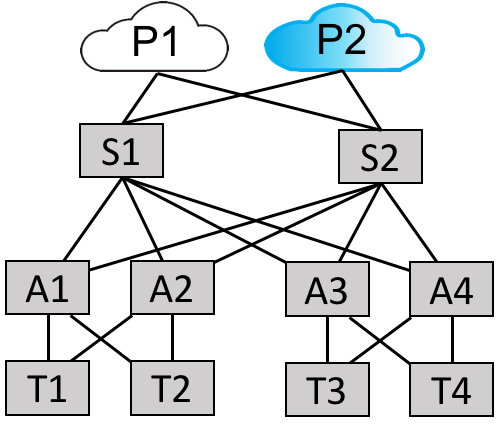
\includegraphics[width=.7\columnwidth]{figures/topology-con}
  \end{minipage}%
  %
  \begin{minipage}[t]{.3\linewidth}
    \hdr{Abstract Topology}{}
    \vspace{1em}
    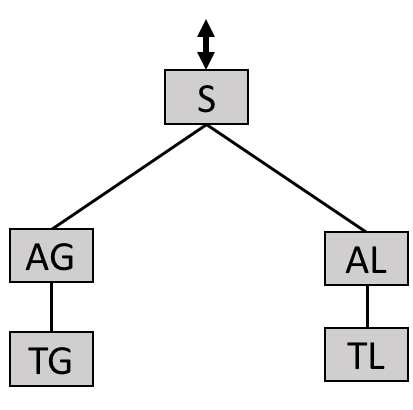
\includegraphics[width=.57\columnwidth]{figures/topology-abs}
  \end{minipage}%

  \vspace{1em}
  \begin{minipage}[t]{.6\linewidth}
    \hdr{Concrete Product Graph}{}
    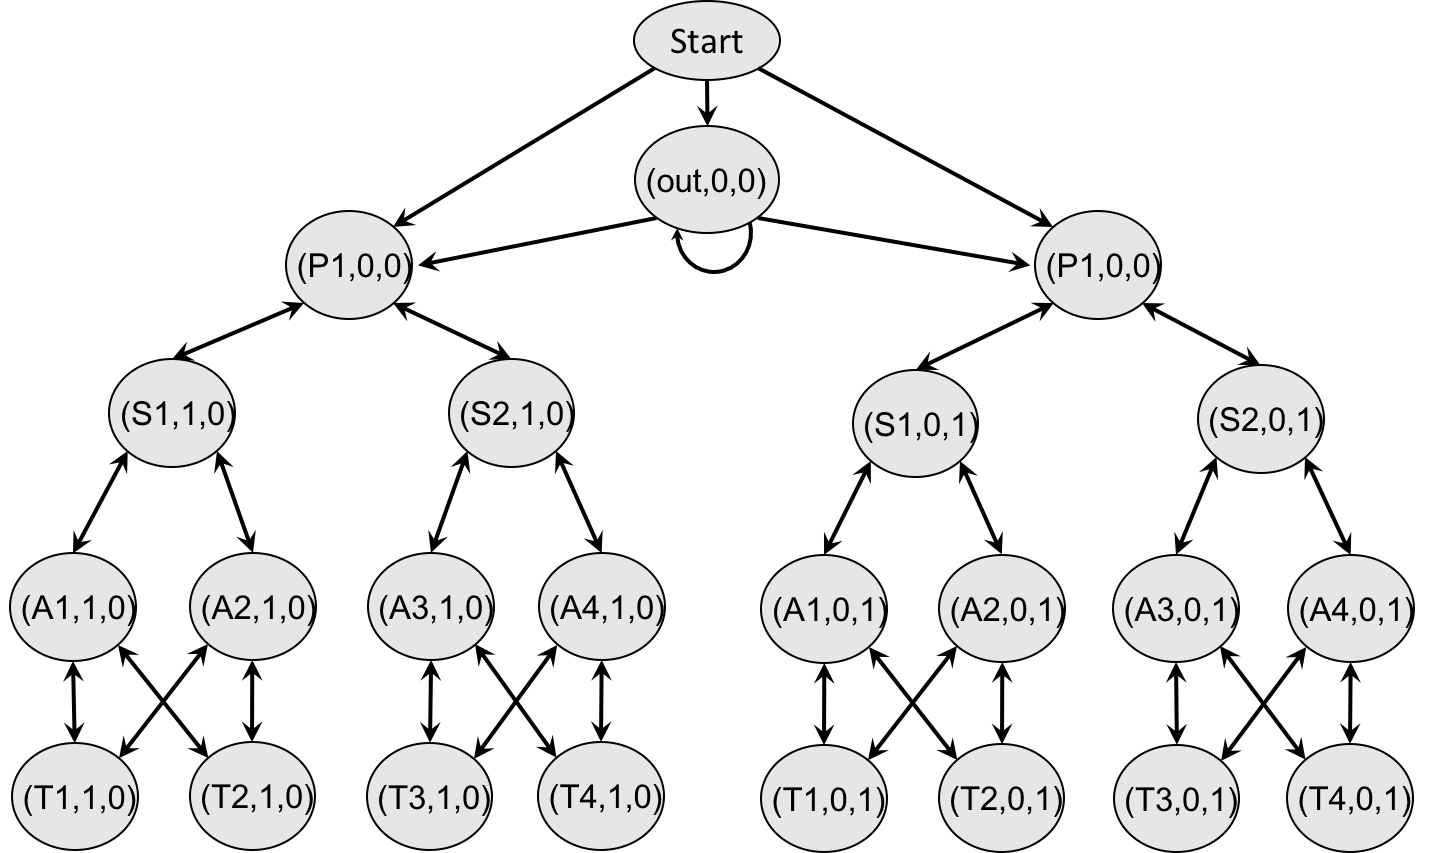
\includegraphics[width=.9\columnwidth]{figures/pg-con}
  \end{minipage}%
  \begin{minipage}[t]{.4\linewidth}
  \hdr{Abstract Product Graph}{}
    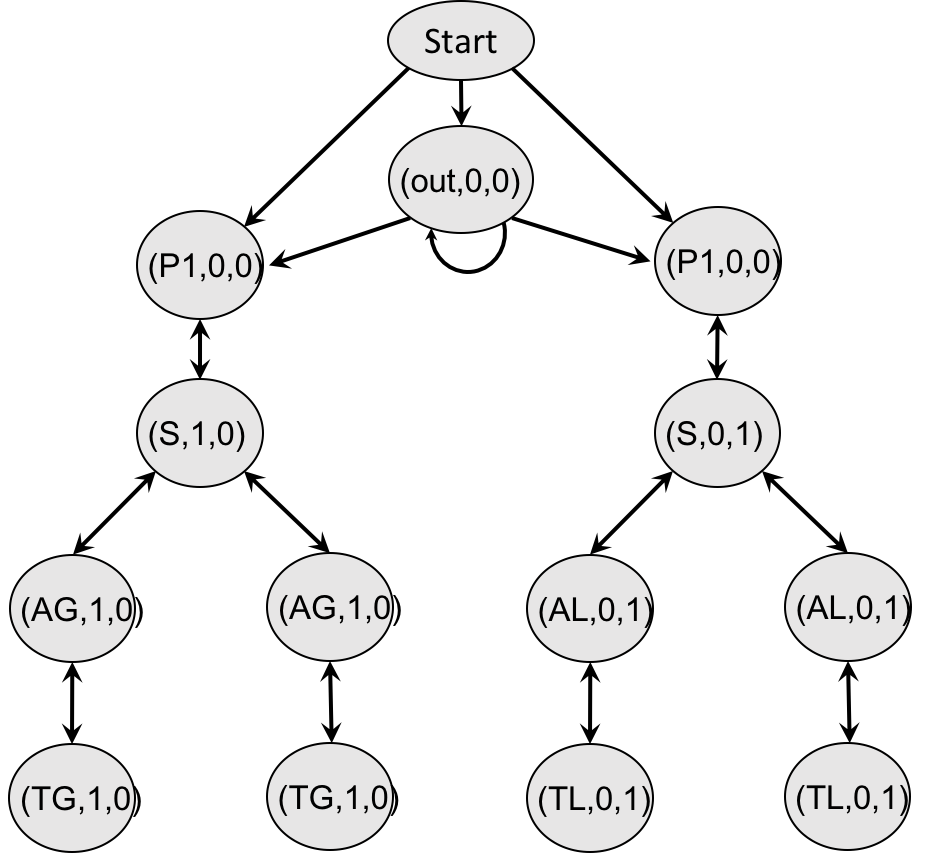
\includegraphics[width=.88\columnwidth]{figures/pg-abs}

  \end{minipage}%

  \hrulefill
  \vspace*{.4em}%

  \caption{Product graph construction for policy $\True ~\Path~ \CD{\Exit(\text{Peer1}} ~\Prefer~ \CD{\text{Peer2})}$.}
  \label{fig:example-compilation}
  %\vspace{-1em}
\end{figure*}


%=====================================================
%
%
%  **Abstractions**
%
%
%=====================================================


\section{Abstract Analysis}
\label{sec:analysis}

In practice, operators would often like to reason about a variety of properties for, not only their current network topology, but also future versions of it.
In this section we present an analysis that operates over the network abstraction to find a lower bound on the number of disjoint paths between pairs of concrete nodes. Answering questions about the number of disjoint paths between nodes allows operators to reason about many useful network properties such as reachability (\IE, is there at least one path) and fault tolerance (\EG, how many failures will disconnect certain routers). Because the analysis takes place over the product graph rather than the topology, it is able to take into account the constraints imposed by the routing policy.


\newcommand{\inference}[7]{
    \node[draw, anchor=west] at (#1 + .5, 2.5 / 2) {#3};
    \node[] at (#1, 2.5 / 2 + 2.5) {\textbf{#5}};
    \node at (#1 + .34, .6 + .2) {#6};
    \node at (#1 + .34, 1.9 - .2) {#7};
    \node at (#1, -.6) {#2};
    \node at (#1, 2.5 + .4 + .2) {#4};
    \draw [] (#1, 2.5 - .2) circle [radius=0.4] node {$n$};
    \draw [] (#1, .2) circle [radius=0.4] node {$m$};
    \draw [->] (#1, .4 + .2) -- (#1, 2.5 - .4 - .2);
}

\newcommand{\inferencenobox}[7]{
    \node[anchor=west] at (#1 + .1, 1.25) {#3};
    \node[] at (#1, 2.5 / 2 + 2.5) {\textbf{#5}};
    \node at (#1 + .34, .6) {#6};
    \node at (#1 + .34, 1.9) {#7};
    \node at (#1, -.6) {#2};
    \node at (#1, 2.5 + .4 + .2) {#4};
    \draw [] (#1, 2.5 - .2) circle [radius=0.4] node {$n$};
    \draw [] (#1, .2) circle [radius=0.4] node {$m$};
    \draw [->] (#1, .2 + .4) -- (#1, 2.5 - .4 - .2);
}

\newcommand{\inferencetwo}[1]{
    \node[draw, anchor=west] at (#1 + 2, 1.25) {$e_i > 0$};
    \node[] at (#1 + .46, 1.25 + 2.5) {\textbf{I-striping}};
    \node at (#1 - 1 - .11, .6) {$e_1$};
    \node at (#1 + .11, 1.5) {$e_2$};
    \node at (#1 + 2 + .11, .6) {$e_3$};
    \node at (#1 + .11 + .8, 1.5) {$e_4$};
    \node at (#1 - 1, -.8) {L$_m(j,k)$};
    \node at (#1 +. 5, 2.9) {S$_n(min(j*k,g),1)$};
    \node at (#1 + 2, -.8) {S$_o\big( min(j, g *\frac{e_4}{e_3}),1\big)$};
    \node at (#1, 3.3) {};
    \draw [] (#1 + .5, 2.01) circle [radius=0.4] node {$n$};
    \draw [] (#1 - 1, 0) circle [radius=0.4] node {$m$};
    \draw [] (#1 + 2, 0) circle [radius=0.4] node {$o$};
    \draw [->] (#1 - 1, .4) -- (#1 + .5, 2 - .4);
    \draw [<-] (#1 + 2, .4) -- (#1 + .5, 2 - .4);
}

\newcommand{\inferencelocal}[2]{
    \node[] at (#1 + 1.2, 2.5 / 2 + 2.5) {\textbf{I-local}};
    \inferencenobox{#1}{L$_m(j,k)$}{}{L$_n(j',k')$}{}{}{}
    \inferencenobox{#1+2 + #2}{$\ldots$ L$_P$ L$_m(j,k)$}{}{$\ldots$ L$_P$ L$_n(j',k')$}{}{}{}
    \node[anchor=east] at (#1 + 2 + #2 - .6, 2.5) {P};
    \draw[dashed] (#1+1 + #2 - .2, -.34) rectangle (#1+3 + #2 + .1, 2.85);
}

\newcommand{\inferenceglobal}[2]{
    \node[] at (#1 + 1.2, 2.5 / 2 + 2.5) {\textbf{I-global}};
    \inferencenobox{#1}{L$_1(j,k)$}{}{L$_2(j',k')$}{}{}{}
    \inferencenobox{#1+2+#2}{$\ldots$ L$_P$ L$_m(j,k)$}{}{$\ldots$ A$_Q$ L$_n(j',k')$}{}{}{}
    \node[anchor=east] at (#1 + 2 + #2 - .6, .4) {P};
    \node[anchor=east] at (#1 + 2 + #2 - .6, 2.5) {Q};
    \draw[dashed] (#1+1+#2 - .2, -.34) rectangle (#1+3+#2 + .1, .8);
    \draw[dashed] (#1+1+#2 - .2, 1.7) rectangle (#1+3+#2 + .1, 2.85);
}

\begin{figure*}[t!]
  \begin{minipage}[t]{\linewidth}%
  \begin{tikzpicture}
    \inference{0}{L$_m(j,k)$}{$e_1 > 0$}{S$_n(min(j*k,e_1),1)$}{I-out1}{$e_1$}{$e_2$}
    \inference{3.5}{A$_m(j,k)$}{$e_2 > 0$}{A$_n(1,min(j,e2))$}{I-out2}{$e_1$}{$e_2$}
    \inference{7}{L$_m(j,k)$}{$e_1=n$}{A$_n(min(j*k,n),1)$}{I-mesh1}{$e_1$}{$e_2$}
    \inference{10.5}{L$_m(j,k)$}{$e_1=n$}{A$_n(1,j)$}{I-mesh2}{$e_1$}{$e_2$}
    \inferencenobox{14}{L$(j,k)$}{$mincut(X)$}{A$(1,min(k,X))$}{I-mincut}{}{}
  \end{tikzpicture}
  \end{minipage}

  \vspace*{1em}
  \begin{minipage}[t]{\linewidth}%
  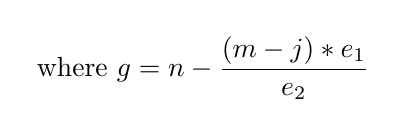
\begin{tikzpicture}
    % \inference{0}{L$(j,k)$}{$e_i > 0$}{S$(min(j*k,g),1)$}{I-out3}{$e_1$}{$e_2$}
    \inferencetwo{0}
    \node[anchor=west] at (1,2.2) {where $g=n-\dfrac{(m-j)*e_1}{e_2}$};
    \inferencelocal{6.5}{.4}
    \inferenceglobal{12}{.4}
  \end{tikzpicture}
  \end{minipage}

  \hrule
  \vspace*{1em}
  \caption{Abstract k-disjoint path analysis inference rules.}
  \label{fig:inference-rules}
  %\vspace{-1em}
\end{figure*}


\subsection{Abstract k-disjoint paths}
\label{sec:property-checking}

In order to infer bounds on the number of disjoint paths between concrete nodes we use information about the structure of the underlying concrete topologies encoded in the abstraction constraints.
%
The idea is to maintain, for each node in the abstract product graph, quantified facts learned about the number of disjoint paths from a source node to some number of concrete routers in that role. More specifically, we maintain facts of the form:
%
\[ \begin{array}{c}
  L_{X_1}, \ldots, L_{X_n}(j,k)
\end{array} \]
\noindent
%
Each label $L \in \{S,A\}$ is either $S$, which stands for ``some" or is $A$, which stands for ``all". There is one label in for each pod label in the abstraction pod hierarchy. For a given node, $L_{X_1}$ would correspond to the outermost pod, $L_{X_{n-1}}$ would correspond to the innermost pod, and $L_{X_n}$ to the the node itself.

Semantically, $L_{X_1}, \ldots, L_{X_n}(j,k)$ means that starting from some concrete router in the abstract source role, for ``some"/``all" pods $X_1$, $L_{X_2}, \ldots, L_{X_n}(j,k)$ holds. The base case $L_{X_n}(j,k)$ means that for ``some"/``all" groups of size $j$ concrete routers, there are $k$ disjoint paths to each such that all $j*k$ paths are disjoint
%
For example, a fact of the form: $A_P, S_{TL}(2,4)$ means that for all pods P, there is some group of 2 concrete routers in role TL such that they each have 4 disjoint paths to them from the source and all 8 paths are disjoint.

\subsection{Inference rules}

\newcommand{\infrule}[1]{{\small \sf #1}\xspace}

In order to learn information about disjoint paths between routers, we develop a series of sound inference rules for facts of this form. Figure~\ref{fig:inference-rules} shows each of the inference rules. The rules are read from bottom to top. The label on the bottom left corresponds to a known fact of the form described above. We use $L$ to represent a rule that is parametric over the particular label ($S$ or $A$). The labels on other nodes correspond to learned facts from applying the inference rule. Conditions that must be \emph{valid} for the rule to apply are shown in a box next to the rule.

In general, the inference rules try to learn information about both the largest number of disjoint paths to any single node in an abstract role and the largest reachable group in a particular role with at least one disjoint path to each.

The first rule, \infrule{I-out1} applies to a learned fact of the form L$(j,k)$ where the number of outgoing edges from any concrete node in the $m$ role is greater than 0. In the worst case, the largest group of concrete nodes we could hope to reach at the $n$ role would be $e_1$ since all j nodes at the bottom may have the same outgoing edges to the concrete nodes at the top. Furthermore, the total number of disjoint paths to the $j$ nodes at the bottom is equal to $j*k$. Since adding edges between the nodes keeps the existing paths disjoint, and since we can not exceed the current number of disjoint paths to the concrete nodes in role $m$ on the bottom, the largest reachable group for the top node will be $min(j*k,e_1)$. However, since we do not know for certain that all $j$ nodes have outgoing edges to the same nodes at the top, we conservatively use $1$ for the number of disjoint paths to each node on top.

The rule \infrule{I-out2} follows a similar line of reasoning. It says that if any group of size $j$ with $k$ disjoint paths to each is reachable in the bottom role, and there is at least one incoming edge for each concrete node in the top role, then there are $min(j,e_2)$ disjoint paths to any single concrete node in the top role. This is because we can choose the $j$ nodes on the bottom for which we want to find disjoint paths, and then use each of the $e_2$ disjoint incoming edges for the particular node at the top connecting it to the bottom.

The two rules \infrule{I-mesh1} and \infrule{I-mesh2} handle the case where there is a full mesh between the two roles. This happens when the number of outgoing edges from the bottom $e_1$ is equal to the number of nodes on the top $n$. The first case for \infrule{I-mesh1} says that we can find disjoint paths to each node in the top role restricted to the number of disjoint paths we started with. The second case for \infrule{I-mesh2} uses the fact that each node in the top role is connected to each node in the bottom role to infer that there can be $j$ disjoint paths to any single node in the top role.

The rule \infrule{I-striping} is the most complicated case.
It starts with the fact L$(j,k)$ at role $m$ and can be applied if each edge multiplicity $e_i > 0$ is valid given the constraints. The first inference for role $n$ tries to find the largest reachable group with disjoint paths to each. The idea is similar to the rule \infrule{I-out1}, but is able to use the fact that $e_2 > 0$ to learn more about the structure of the concrete topology. In particular it uses the following inequality, where $g$ represents the size of the group for the role $n$:
%
\[ \begin{array}{c}
  (m-j)*e_1 \geq (n-g)*e_2
\end{array} \]
\noindent
%
This captures the fact that the remaining nodes ($m-j$) that are not part of the group in the bottom role, each have $e_1$ outgoing edges and must be able to at least "fill" the incoming edges for the remaining nodes not in the reachable group at the top ($n-g$) with $e_2$ incoming edges each. Solving the inequality yields:
%
\[ \begin{array}{c}
  g \geq n - \dfrac{(m-j)*e_1}{e_2}
\end{array} \]
\noindent
%
The second part of the rule allows uses a similar idea to reason about the overlap between roles $m$ and $o$ with respect to role $n$. This rule is useful particularly useful for datacenter topologies where routers in one tier of the datacenter often have a particular striping pattern with another tier.

The rule \infrule{I-mincut} can be thought of as an assertion about the fault tolerance between two roles. The rule applies to an edge that has been annotated with a $mincut(X)$ statement, which means that there are at least $X$ disjoint paths between any node in role $m$ and any node in role $n$. 

Finally, the \infrule{I-local} and \infrule{I-global} rules allow us to lift each of the other rules to reason across pod hierarchies. The first rule, \infrule{I-local}, says that if you have an inference from L$_m(j,k)$ to L$_n(j',k')$ on the left, then if both nodes are in the same local pod P, you can leave all labels up to P unchanged. The global rule \infrule{I-global} says the same thing except when the edge goes between pods, you can infer the fact for all pods Q since the multiplicities apply equally to each pod.

\subsection{An inference algorithm}

The abstract disjoint path analysis starts from a fixed source location $src$ and repeatedly applies the inference rules from Figure~\ref{fig:inference-rules} until it reaches a fixed point. Inference rule conditions can be checked for validity over all concrete topologies using an SMT solver. In order to ensure termination, we make the observation that, for any fact learned of the form $L(j,k)$, it is sound to instead infer $L(j',k')$ if $j' \leq j$ and $k' \leq k$. Therefore, for each inference rule that learns a fact of the form $L(j,k)$ we minimize the symbolic expressions for $j$ and $k$ subject to the topology constraints using the optimization framework $\nu$Z~\cite{z3opt}.

\begin{figure}
  \begin{center}
    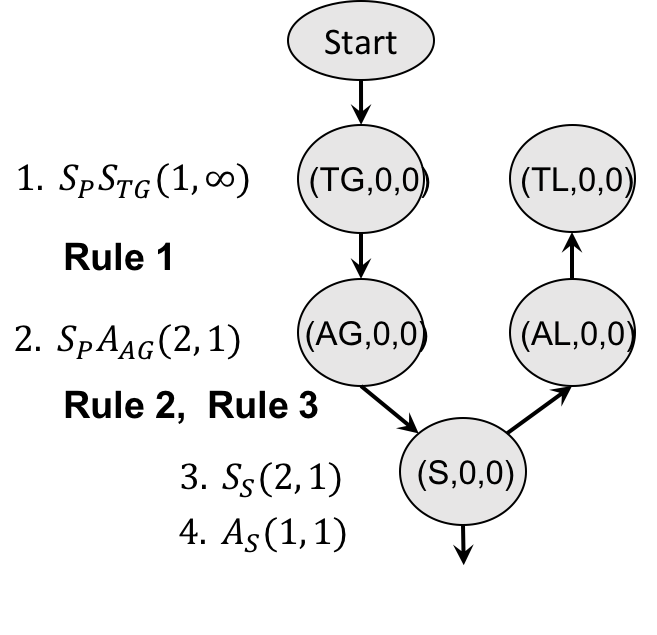
\includegraphics[width=\columnwidth]{figures/analysis}
  \end{center}
  \caption{Abstract disjoint path analysis with valleyfree routing for global prefixes. \label{fig:compilation-times}}
  \label{fig:example-inference}
  \vspace{-1em}
\end{figure}

Consider again the datacenter example from \S\ref{sec:overview}. Suppose now we add the valleyfree constraint that traffic never takes a path with a down-up in it for the routing policy for global prefixes:
%
\begin{code}
\$GP \Path \End(TG) \ensuremath{\cap} \Novalley(\{TG,TL\},\{AG,AL\},\{S\})
\end{code}
\noindent
%
Figure~\ref{fig:example-inference} shows the abstract product graph representation for this routing policy. The inference algorithm starts from the node $(TG,0,0)$ with the initial fact $S_P S_{TG}(1,\infty)$ (\IE, no restriction on the number of disjoint paths initially).
%
The first step applies the rule \infrule{I-mesh1} together with \infrule{I-local} to reason about connectivity within a single pod for the TG and AG roles. This invokes a call to $\nu$Z to minimize the expression $min(\infty, AG)$, which results in 2. Therefore, the algorithm learns a new invariant of the form $S_P A_{AG} (2,1)$ for node $(AG, 0)$ to indicate that in some pod P, any group of 2 nodes is reachable.
%
The next step uses the inference rule \infrule{I-out2} to learn that any single spine node is reachable. It also can apply rule \infrule{I-striping} to determine that there is some group of at least 2 spine routers reachable at node $(S,0)$ and also that there is some group of at least 2 nodes reachable in the AL role in state $(AL,0)$.

Note that, because each inference rule only applies to directed edges in the product graph, the algorithm can not make any inferences about connectivity from the AL role to the S role since there is no directed edge between them. It is this restriction that ensures that the analysis is both topology and policy dependent.

The next step is to use \infrule{I-mesh2} together with \infrule{I-local} to infer than any single node in the TL role for any pod P is reachable via at least 2 disjoint paths. This process will continue until a fixed point is reached.

In this case, the algorithm was able to infer that, with the valleyfree routing policy, any node in the spine role has at least 1 disjoint path and any node in the TL node has at least 2 disjoint paths to a router in role TG. Note that, in this case, the analysis is precise. There exists a concrete network, namely the datacenter from Figure~\ref{fig:example2}, where a single failure can disconnect a global tor from a spine router due to the valleyfree constraint. In this case, a bound on the fault tolerance between a tor and spine router can be used to ensure that an aggregation-induced black hole will not occur at the border of the datacenter until a certain number of failures occur.


%=====================================================
%
%
%  **Compilation to BGP**
%
%
%=====================================================

\newcommand{\highlight}[1]{%
  \colorbox{red!50}{$\displaystyle#1$}}
\newcommand{\Router}[1]{\KW{Router} #1:}
\newcommand{\Template}[1]{\KW{Template} #1:}
\newcommand{\REGEX}[1]{\texttt{regex}(#1)}
\newcommand{\PEER}{\texttt{peer}}
\newcommand{\PREFIX}{\texttt{prefix}}
\newcommand{\IF}{\texttt{if}}
\newcommand{\THEN}{\texttt{then}}
\newcommand{\COMM}{\texttt{comm}}
\newcommand{\MED}{\texttt{MED}}
\newcommand{\Arrow}{\ensuremath{\leftarrow}}

\begin{figure}[t!]
  \begin{code}
    \Template{S}
      Match[100] \PREFIX=\$GP, \PEER=\{AG, AL\}
        \PEER \Arrow *
      Match[100] \PREFIX=\$LP, \PEER=\{AG, AL\}
        \PEER \Arrow \{AG, AL\}
      Match[110] \PREFIX=true \PEER=\{P1\},
        \PEER \Arrow *, \COMM \Arrow (1,0)
      Match[100] \PREFIX=true \PEER=\{P2\},
        \PEER \Arrow *, \COMM \Arrow (0,1)
      ...
  \end{code}

  \vspace{-2em}
  \begin{code}
    \Router{S1, S2}
      Match[100] \PREFIX=GP1, \PEER=\{AG1, AL1, ...\}
        \PEER \Arrow *
      Match[100] \PREFIX=GP2, \PEER=\{AG1, AL1, ...\}
        \PEER \Arrow *
      ...
      Match[100] \PREFIX=LP1, \PEER=\{AG1, AL1, ...\}
        \PEER \Arrow \{AG1, AL1, ...\}
      Match[100] \PREFIX=LP2, \PEER=\{AG1, AL1, ...\}
        \PEER \Arrow \{AG1, AL1, ...\}
      ...
      Match[110] \PREFIX=true, \PEER=\{P1\},
        \PEER \Arrow *, \COMM \Arrow (1,0)
      Match[100] \PREFIX=true, \PEER=\{P2\},
        \PEER \Arrow *, \COMM \Arrow (0,1)
      ...
    \end{code}

  \vspace{-1em}
  \caption{Spine template and concrete configurations.}
  \label{fig:bgp-configs}
\end{figure}


\section{Compilation}

The translation from the Product Graph to per-device configurations that run the distributed BGP protocol involves several ideas.

\para{Route filtering}

The first idea is to tag every protocol message with a BGP community value that encodes the state of each automaton when advertising a route to a neighbor. Routers can then allow route advertisements that correspond to an edge in the Product Graph and block those that don't.
%This ensures that any path computed by BGP will be a valid path in the Product Graph, and thus is allowed by the policy.
For example, in the concrete Product Graph in figure~\ref{fig:example-compilation}, router $S1$ will allow a route advertisement from its neighbor $P1$ and also from neighbor $P2$. If it uses the path provided by neighbor $P1$, then it will add the tag $(1,0)$ before informing its neighbors about this route. On the other hand, if it uses neighbor $P2$, then it will add the tag $(0,1)$ instead.


\para{Preference Search}
The second idea is to have each router totally order advertisements from neighbors. For example, to satisfy the policy that leaving through $\sf{P1}$ is preferred to leaving through $\sf{P2}$, router $S1$ should prefer a message it hears from $P1$ over one from $P2$. Similarly, router $A1$ should prefer routes tagged with $(1,0)$ over those tagged with $(0,1)$.
%In general, because BGP is distributed, each router does not have a full view of the entire network when choosing which path to use. Because finding a collection of preferences to ensure correct end-to-end behavior for all failures is a hard problem,
Propane introduced a conservative, yet effective algorithm for determining route preferences based on the following observation about the structure of the Product Graph:

\begin{defn}
Let $m \geq_{rank} n$ be a relation over Product Graph vertices that holds iff $P(n) = \emptyset$ or $\min P(m) \geq \min P(n)$. Intuitively $m \geq_{rank} n$ means that paths ending at PGIR node $m$ are no better than paths ending at $n$.
%
\end{defn}
\noindent
%

%\begin{defn}
The product graph can be viewed as a labelled transition system by pushing the location from each directed edge's target node onto the edge. That is, $m\overset{l}{\rightarrow}n$ if edge $(m,n) \in E'$ and $\tilde{n} = l$.
%\end{defn}
%
For example, in the concrete product graph we would have the transition $(S1,1,0)\overset{A2}{\rightarrow}(A2,1,0)$.

\begin{defn}
We write $m \leq m'$ if the subgraph reachable from $m$ and $m'$ respectively form a simulation relation with respect to the $\geq_{rank}$ relation.
\end{defn}

If each router has a total order with respect to the simulation relation ($\leq$) for its corresponding Product Graph nodes, then we simply sort the nodes and prefer advertisements from peers of node $m$ over those of node $m'$ if $m' \leq m$.
%
For example, in the concrete product graph the inequality $(S1,0,1) \leq (S1,1,0)$ holds since nodes on the left side of the product graph can always match transitions made on the right hand side with respect to the $\geq_{rank}$ relation. This relation does not hold the other way around since $(S1,0,1) \ngeq_{rank} (S1,1,0)$. Therefore, advertisements received at $S1$ in state $(1,0)$ must be preferred to those received in state $(0,1)$.

Notice also that in the abstract product graph the inequality $(S,0,1) \leq (S,1,0)$ holds. This leads us the the following observation:

\begin{lem}
\label{lem:preference}
$m \leq m'$ in the concrete product graph iff $f_{pg}(m) \leq f_{pg}(m')$ in the abstract product graph under the lifted graph homomorphism $f_{pg}$.
\end{lem}

Lemma~\ref{lem:preference} gives us reason to believe that we can perform compilation over the abstract product graph and ensure that the inferred device-level preferences will be correct when instantiating the template with a concrete network.



\para{BGP configurations}

%By combining the tagging, filtering and preference mechanisms, we can generate safe BGP configurations. In general, configurations are generated by combining the per-prefix configurations in the same order specified in the policy.
Figure~\ref{fig:bgp-configs} shows part of the final configuration for spine routers for the concrete and abstract policies.
%
For prefix $0.0.0.0/[0..32]$, the spine routers will match advertisements from peer $P1$ and $P2$. The match for $P1$ is preferred since it has a higher BGP local-preference attribute (110). If an advertisement from $P1$ is available the spine uses this and attaches the community tag $(1,0)$ and advertises the route to all its peers. If only an advertisement from the backup $P2$ is available, then it attaches the tag $(0,1)$ and advertises this to all peers instead.
%
There is also additional policy for the Product Graphs from constraints for the local and global prefixes. In the template configuration, it matches any global prefix from any internal peer and re-advertise the route to all of its peers. For any local prefix it will allow an advertisement from any internal peer, and re-advertise the route to only other internal peers (thus implementing the Local constraint). The concrete configurations have a similar configuration for each local and global prefix.



%=====================================================
%
%
%  **Concretization**
%
%
%=====================================================

\newcommand{\Con}{\text{con}}
\newcommand{\Pfx}{\mathit{pfx}}%

%\vspace{2em}
%\begin{figure*}[t!]\small%

%  \hrulefill%
%  \vspace{1em}%

%  \begin{minipage}[t]{.46\linewidth}
%  \hdr{ABGP Syntax}{}
%  \vspace*{-1\baselineskip}
%  %
%  \[ \begin{array}{rclr}
%     d    &   & & \textit{integer} \\
%     c    &   & & \textit{community} \\
%     t    &::=& \$x \BNFALT d.d.d.d/[d..d] & \textit{predicate} \\
%     ns   &::=& \{ l_1, ~\dots,~ l_k \} & \textit{peers} \\
%     ma   &::=& d : ({ns}_1, c_1) \rightarrow ({ns}_2, c_2) & \textit{match action} \\
%     pc   &::=& ma_1, \dots, ma_k & \textit{prefix config} \\
%     rc   &::=& t_1 \rightarrow {pc}_1, ~\dots,~ t_k \rightarrow {pc}_k & \textit{router config} \\
%     abgp &::=& l_1 \rightarrow {rc}_1, ~\dots,~ l_k \rightarrow {rc}_k & \textit{abgp policy} \\%

%  \end{array} \]%%

%  \end{minipage}
%  %
%  %
%  \begin{minipage}[t]{.5\linewidth}
%  \hdr{Compilation}{}
%  \vspace*{-1\baselineskip}
%  %
%  \[ \begin{array}{l}
%     \text{compile}_\text{ABGP}( (t_1,PG_1,ord_1), \dots, (t_k,PG_k,ord_k), G ) = \\
%     ~~~~~ [~ l \rightarrow rc ~\vert~ \\
%     ~~~~~~~~~ l \in internal(G.V), \\
%     ~~~~~~~~~ rc = \mathit{append}_i~  \\
%     ~~~~~~~~~~~~~~~ [~ t_i \rightarrow ma_1, \dots, ma_k ~\vert~ \\
%     ~~~~~~~~~~~~~~~~~~~~~ m = (l,q_m) \in PG_i, \\
%     ~~~~~~~~~~~~~~~~~~~~~ pin = \text{adjIn}(PG_i,m), \\
%     ~~~~~~~~~~~~~~~~~~~~~ (in,q_n) = \{ (bs,q_n) ~\vert~ (\_,q_n) \in pin, bs=\{b ~\vert~ (b,q_n) \in pin \} \} \\
%     ~~~~~~~~~~~~~~~~~~~~~ out = \{ c ~\vert~ (c,\_) \in \text{adjOut}(PG_i,m) \} \\
%     ~~~~~~~~~~~~~~~~~~~~~ ma_j = ord_i(m) : (in,q_n) \rightarrow (out,q_m) ~] ~] \\
%     \\
%     \text{compile}( p_1, \dots, p_k, G) = \\
%     ~~~~~~ \text{compile}_\text{ABGP}(\text{compile}_\text{PG}(p_1,G), \dots, \text{compile}_\text{PG}(p_k,G), G) \\
%  \end{array} \]%
%  \end{minipage}%

%  \vspace{1em}
%  \vspace{1em}%

%  \vspace*{-2\baselineskip}
%  \begin{minipage}[t]{1.01\linewidth}
%  \hdr{Policy Concretization}{}
%  \vspace*{-2\baselineskip}
%  %
%  \[ \begin{array}{lcl}
%     \\
%     \Con(\emptyset, \Gamma, f)      &=& \emptyset \\
%     \Con(l, \Gamma, f)              &=& \Sigma_i ~ f_i^{-1}(l) \\
%     \Con(r_1 \cup r_2, \Gamma, f)   &=& \Con(r_1,\Gamma,f) \cup \Con(r_2,\Gamma,f) \\
%     \Con(r_1 \cap r_2, \Gamma, f)   &=& \Con(r_1,\Gamma,f) \cap \Con(r_2,\Gamma,f) \\
%     \Con(!r, \Gamma, f)             &=& !\Con(r,\Gamma,f) \\
%     \Con(r^*, \Gamma, f)            &=& \Con(r,\Gamma,f)^* \\%

%     \Con(\Pfx ~\Path~ r_1, ~\dots~, r_k, \Gamma, f) &=&
%          \Pfx ~\Path~ \Con(r_1,\Gamma,f), ~\dots~, \Con(r_k,\Gamma,f)  \\%

%     \Con(\$x ~\Path~ r_1, ~\dots~, r_k, \Gamma, f) &=&%

%         [~ \Pfx ~\Path~ \Con(r_1,\Gamma,f) \cap \text{end}(l), ~\dots~, \\%

%         & & ~~~~~~~~~~~~~~~ \Con(r_k,\Gamma,f) \cap \text{end}(l) ~\vert~ (\Pfx,l) \in \Gamma(x) ~]  \\%

%     \Con(p_1, \dots, p_n, \Gamma,f) &=& \Con(p_1, \Gamma,f), \dots, \Con(p_n, \Gamma,f) \\%

%  \end{array} \]%
%  \end{minipage}%

%  \vspace{1em}
%  \vspace{1em}%

%  \begin{minipage}[t]{\linewidth}
%  \hdr{ABGP Concretization}{}
%  \vspace*{-2\baselineskip}
%  %
%  \[ \begin{array}{lcl}
%     \\
%     \Con(l_1 \rightarrow {rc}_1, ~\dots,~ l_k \rightarrow {rc}_k,\Gamma,f,G)
%        & = &
%        \mathit{append}_i~ [~ \ell \rightarrow con(rc_i,\ell,\Gamma,f,G)  ~\vert~ \ell \in f^{-1}(l_i) ~]
%        \\
%     \Con(t_1 \rightarrow {pc}_1, ~\dots,~ t_k \rightarrow {pc}_k,\ell,\Gamma,f,G)
%        & = &
%        \Con(t_1 \rightarrow {pc}_1,\ell,\Gamma,f,G), \dots, \Con(t_k \rightarrow {pc}_k,\ell,\Gamma,f,G)
%        \\
%     \Con(\Pfx \rightarrow {pc},\ell,\Gamma,f,G)
%        & = &
%        \Pfx \rightarrow \Con(pc,\text{true},\ell,\Gamma,f,G)
%        \\
%     \Con(\$x \rightarrow {pc},\ell,\Gamma,f,G)
%        & = &
%        [~ \Pfx \rightarrow \Con(pc, l=\ell, \ell,\Gamma,f,G) ~\vert~ (\Pfx, l) \in \Gamma(x) ~]
%        \\
%     \Con(ma_1, \dots, ma_k,o,\ell,\Gamma,f,G)
%        & = &
%        \Con(ma_1,o,\ell,\Gamma,f,G), \dots, \Con(ma_k,o,\ell,\Gamma,f,G)
%        \\%

%     \Con(n_1 : ({ns}_1, n_2) \rightarrow ({ns}_2, n_3),o,\ell,\Gamma,f,G)
%        & = & \textbf{if}~ ns_1 = \{\text{start}\} ~\text{and}~ o = \text{false} ~\textbf{then}~ \bullet \\
%        &   & \textbf{else}~ n_1 : ( \Con({ns}_1,\ell,\Gamma,f,G), n_2) \rightarrow (\Con({ns}_2,\ell,\Gamma,f,G),n_3)%

%        \\
%     \Con(\{ l_1, ~\dots,~ l_k \}, \ell, \Gamma,f,G)
%        & = &
%        \bigcup_i ~ \{ x ~\vert~ x \in f^{-1}(l_i),~ (x,\ell) \in G.E \}
%        \\
%  \end{array} \]%
%  \end{minipage}%

%  \vspace{1em}
%  \hrulefill%
%  \vspace{1em}%

%  \caption{ABGP syntax, compilation from product graphs, policy concretization, and ABGP concretization.}
%  \label{fig:concretization}
%\end{figure*}%




\section{Concretization}

One interesting observation is that the spine template configuration and concrete spine configurations are structured similarly. In this section, we formalize this observation. We introduce a simple language for BGP configurations called ABGP and define compilation policies over both concrete and abstract topologies to ABGP. In addition we define a concretization function for that translates an abstract \sysname policy or ABGP configuration to a concrete \sysname policy or ABGP configuration respectively. The main result is that the compilation and concretization functions commute. This means performing compilation over the abstract representation first allows us to generate templates, and only concretize these templates when we need to instantiate the network.

%\para{ABGP language}%

%We introduct a simple language for BGP configurations called ABGP. Figure~\ref{fig:concretization} shows the syntax for an ABGP policy. An ABGP policy maps topology locations $l$ to router configurations $rc$. Each router configuration $rc$ is a sequence of predicates $t$ and their corresponding configuration $pc$. A prefix configuration $pc$ is a sequence of match actions. Each match action $ma$ consists of a preference value $d_1$, followed by a set of imports from neighbors $ns_1$ and community value (\IE, state of the product graph) $d_2$ expected from those neighbors, as well as export neighbors $ns_2$ and the community value $d_3$ to attach before sending to those neighbors.%
%

%\para{Compilation}%

%Figure~\ref{fig:concretization} defines compilation from a \sysname policy to an ABGP policy. It starts by compiling ($\text{compile}_\text{PG}$) separately each constraint of the form $p_i = (t_i ~\Path~ r_{i1} ~\Prefer~ r_{ik})$ to a product graph $PG = (G', s, P)$. The function $\text{compile}_\text{PG}$ returns the test $t_i$, product graph $PG_i$, and the preference ordering $ord_i$.
%%
%The function $\text{compile}_\text{ABGP}$ then takes a sequence of tuples $(t_i, PG_i, ord_i)$ and returns an ABGP policy. For each internal router, it looks at each set of neighbor with the same community state $q_n$ and matches any of those neighbors with the preference provided by the ordering $ord$. It then exports this advertisement to each adjacent peer along an outgoing edge and adds the community value for the current state $q_m$.%

%%We assume a particular router $l$ appears at most once in any abgp specification.
%We build configs using set-builder notation.  For instance,
%$\{l \rightarrow rc ~\vert~ l \in V \wedge p(l,rc)\}$ denotes the abgp policy
%%
%\[ \begin{array}{c}
%  l_1 \rightarrow rc_{1},... \\
%  ...           \\
%  l_k \rightarrow rc_{k},... \\
%\end{array} \]


%where $l_1, ..., l_k$ are the nodes in the topology
%and each $rc_{i}$ satisfies $p(l_i,rc_{i})$. We also use the $\bigcup$ operator to denote sequence concatenation.%

%\para{Concretization}%

%Concretization for a \sysname policy takes as input, the policy and a context
%$\Gamma : Var \rightarrow 2^{Prefix \times V}$,
%which maps from a template prefix to a set of pairs of a concrete prefix and a concrete location that "owns" the prefix.
%%
%For each regular expression $r$, we replace each abstract location with the sum over its corresponding concrete locations under the inverse homomorphism $f^{-1}$. For each template variable, we replace it with a new entry for each of its corresponding concrete prefixes under the supplied mapping $\Gamma$. We also intersect the resulting concretized regular expression with $\text{end}(l)$ to capture the fact that this traffic is owned by the concrete location $l$.%

%We also define concretization over the ABGP policy in a similar manner. We replace each abstract router configuration $l \rightarrow rc$ a new entry for each concrete location $\ell \in f^{-1}(l)$. The concrete location $\ell$ is passed as a parameter to $con$ to remember the current router.
%%
%To concretize a prefix policy with a template ($\$x \rightarrow pc$) we replace it with a sequence of policies, one for each prefix in context ($(pfx,l) \in \Gamma(x)$). Match action statements where the set of import neighbors is the singleton set containing the product graph start node $\{ start \}$ and we are not currently at looking at the router configuration for the location specified in the context $l$, then we drop the match action. This is denoted with the $\bullet$ symbol. Finally, to concretize a set of neighbors, we again use $f^{-1}$ to find the set of concrete neighbors under the inverse homomorphism, but then restrict it to those that are actually connected in the underlying concrete topology with $G.E$.


\begin{thm}
  For any context $\Gamma$, topology $G$, abstract topology $G^A$, homomorphism $f : G \rightarrow G^A$, and policy $pol$,
  $$\Con(\text{compile}(pol,G^A), \Gamma,f,G) = \text{compile}(\Con(pol,\Gamma,f),G)$$
\end{thm}

\subsection{Incrementality}

Suppose that we want to expand our example concrete datacenter by adding an additional tor router in the TG role. Per the network routing policy, this new tor router will advertise its new owned prefix. Because the new topology matches the abstraction, the compiled templates will remain the same. However, in the spine router configurations, the match on the global prefix template variable \$GP will be expanded to include the new prefix owned by the added tor. In other words, the concrete configurations obtained after substitution will include an additional match on the new prefix. Unfortunately, this means that a small change to the topology can result in many configurations far from the change needing to change too.

The key insight is that the template variables tell us exactly where change can happen. For example, the only way in which the spine routers depend on anything non-local is in the match on prefix template variables. Instead, we can associate a new unique community tag for each template variable like \$GP. We can replace each match on \$GP with a test on the new community tag. The new added tor will now simply attach the new community tag to advertisements for its prefix so downstream routers can just match the community tag. This ensures that each router has a template that has no dependency on any other non-adjacent router. If we make a change to the concrete network that matches the abstraction, then the templates do not change, and thus only configurations adjacent to the changes must also change.




%=====================================================
%
%
%  **Implementation and Evaluation**
%
%
%=====================================================


\section{Implementation and Evaluation}
\label{sec:evaluation}

The \sysname compiler is implemented in approximately 9500 lines of F\# code. The compiler accepts both concrete and abstract topologies and will generate router configurations for open-source Quagga routers. Operators can specify their required fault tolerance level for aggregation safety. The abstract safety analysis uses $\nu$Z~\cite{z3opt} test validity and to minimize variables subject to the annotated constraints. Since the analysis typically calls the SMT solver with many times with relatively simple optimization problems, we use a timeout of 200ms.

Although the disjoint path analysis takes place over the Product Graph, each application of the inference rules from figure~\ref{fig:inference-rules} depends only on the topology. Therefore, we lazily apply the rules and cache the satisfiability and minimization calls to $\nu$Z after their first use. Furthermore, the cached results are shared across different prefixes, each of which may have a unique Product graph representation.

To evaluate \sysname, we apply it on policies for backbone and datacenter networks. We aim to evaluate the expressiveness of our abstract multiplicity annotations, the precision of the abstract disjoint-path analysis, and the compilation time of \sysname both with abstraction and without.

\subsection{Analysis precision}

\begin{figure}[t!]
  \begin{center}
      \begin{tabular}{| l | c | c | c |}
      \hline
      \textbf{Topology} & \textbf{Fixed} & \textbf{Reachable} & \textbf{K-paths} \\ \hline
      Fattree~\cite{fattree} & & \cmark & \cmark  \\ \hline
      Facebook~\cite{facebook-fattree} & & \cmark & \cmark \\ \hline
      F10~\cite{f10-fattree} & & \cmark & \cmark \\ \hline
      VL2~\cite{vl2-fattree} & & & \\ \hline
      BCube~\cite{bcube} & $k$ & \cmark & \xmark \\ \hline
      DCell~\cite{dcell} & $k$ & \cmark & \xmark \\ \hline
         %& HCN & $h$ & \cmark & \xmark \\
      Butterfly~\cite{butterfly} & $n$ & \cmark & \cmark \\ \hline
      Hypercube & $N$ & \cmark & \cmark \\ \hline
      HyperX~\cite{hyperx} & $L$ & \cmark & \cmark \\ \hline
      \end{tabular}
  \end{center}
  \caption{Abstract Analysis Precision.}
  \label{fig:analysis-precision}
\end{figure}

%\begin{figure}[t!]
%  \begin{center}
%      \begin{tabular}{| l l | c | c | c |}
%      \hline
%      \textbf{Topology} & \textbf{Variant} & \textbf{Fixed} & \textbf{Reachable} & \textbf{K-paths} \\ \hline
%      Fattree
%         & Google &  & \cmark & \cmark  \\
%         & Facebook &  & \cmark & \cmark \\
%         & F10 &  & \cmark & \cmark \\ \hline
%      Recursive
%         & BCube & $k$ & \cmark & \xmark \\
%         & DCell & $k$ & \cmark & \xmark \\ \hline
%         %& HCN & $h$ & \cmark & \xmark \\
%      Hypercube
%         & Standard & $N$ & \cmark & \cmark \\
%         & HyperX & $L$ & \cmark & \cmark \\ \hline
%      Random \footnote{foo}
%         & Scafida &  & ??? & ??? \\
%         & JellyFish &  & ??? & ??? \\
%      \hline
%      \end{tabular}
%  \end{center}
%  \caption{Abstract Analysis Precision.}
%  \label{fig:analysis-precision}
%\end{figure}

We evaluate the expressiveness and precision of our abstract analysis on a range of different network topologies found in both the network literature and production. For each topology in figure~\ref{fig:analysis-precision} we define a suitable abstraction. Since many topologies have tunable parameters (e.g., the recursion depth $k$ for the DCell topology), we list all such parameters that are fixed for our abstraction. We implement a shortest path routing policy over the topology and record the precision of the abstract analysis in terms of whether or not it is able to accurately prove reachability and/or the correct number of disjoint paths between all pairs of nodes.

\para{Fat Tree Topologies}

The Fat Tree topology is one of the most widely used datacenter topologies. We look at the precision of our analysis on four variants of the Fat Tree topology used in practice: a Standard Fat Tree~\cite{fattree}, the Facebook Fat Tree~\cite{facebook-fattree}, the F10 fault tolerant Fat Tree~\cite{f10-fattree}, and the VL2 topology~\cite{vl2-fattree}. For each Fat Tree variant, we use a tiered abstraction similar to that in our previous example. Each Fat Tree topology is parameterized over the number of pods $k$, which can be scaled up in the abstraction to allow for expansion. For all Fat Tree variants, the analysis is precise enough to determine the exact number of disjoint paths between all pairs of concrete routers.

\para{Recursive Topologies}

We also model several recursive topologies using our abstractions. These include the BCube~\cite{bcube} and Dcell~\cite{dcell} topologies. Each topology includes a recursion depth parameter ($k$), which we must fix. For a recursive topology with depth $d$, we model it as an abstract topology consisting of abstract nodes for each of the depth $d-1$ subcomponents. This allows for safe expansion within a subcomponent, but not from increasing the recursion depth. The analysis is able to accurately determine reachability (i.e., at least 1 disjoint path) for each recursive topology, but is overly conservative in determining k-disjoint paths. For the BCube topology, it is able to to determine the correct number of disjoint paths between some pairs of nodes, but not all.

\para{Hypercube Topologies}

Hypercube variants can be used as an alternative to Clos-style topologies for networks with high-radix (port density) routers. The HyperX~\cite{hyperx} topology can be viewed as a generalization of the hypercube and butterfly topologies, which includes parameters $L$ for the lattice dimension of the network, $S_i$ for the node multiplicity of each dimension $i$, $K_i$ for the bandwidth of links for each dimension, and $T$ for the number of terminal nodes (servers) connected to each router. For a fixed number of dimensions $L$, we abstract each full mesh of $S_L$ nodes into its own abstract node. The $S_{x-1}$ groups of abstract nodes can be captured using pods of the abstract $S_x$ nodes.

%\para{Random Network Topologies}
%
%Random networks such as Scafida and Jellyfish have seen a great deal of interest in academia. These topologies were designed with an eye towards incremental expansion and are based on probabilistic arguments of bisection bandwidth in random regular graphs. However, because the topologies are created randomly, there are no hard guarantees on the connectivity between different routers. We can trivially represent these networks using a \emph{one big router} abstraction for the entire network.


\subsection{Compilation time}

\begin{figure}[t!]
  \subcaptionbox{Datacenter}
    {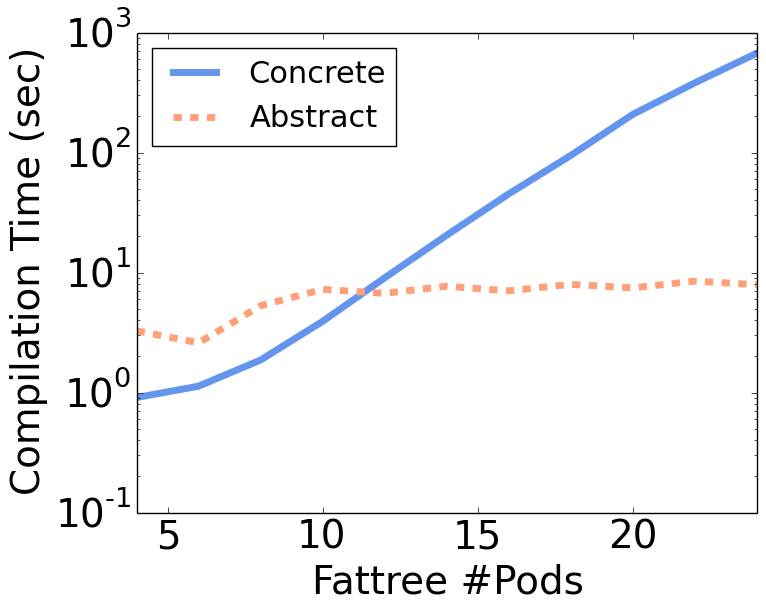
\includegraphics[width=.49\columnwidth]{figures/Fattree-time.png}}
  \subcaptionbox{Backbone}
    {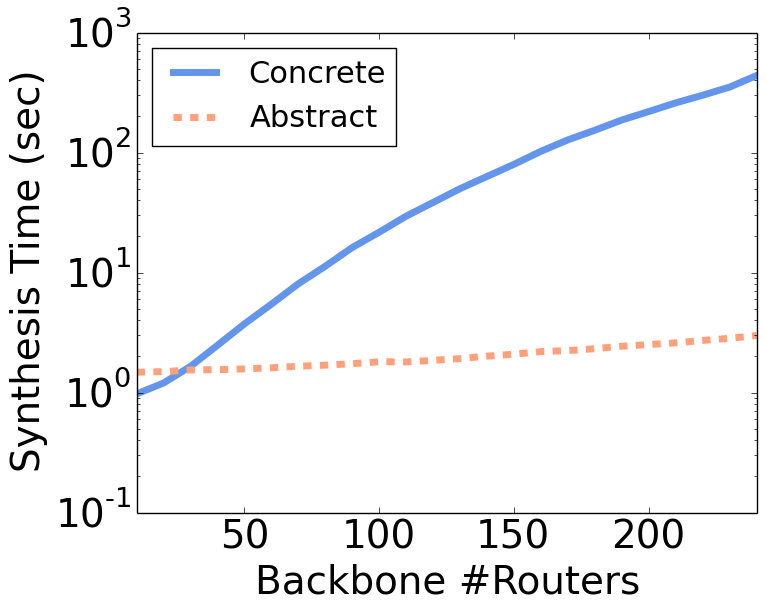
\includegraphics[width=.49\columnwidth]{figures/backbone-time.png}} \\
  \caption{Concrete vs. Abstract Compilation Time. \label{fig:compilation-times}}
  \vspace{-1em}
\end{figure}

\begin{figure}[t!]
  \subcaptionbox{Datacenter}
    {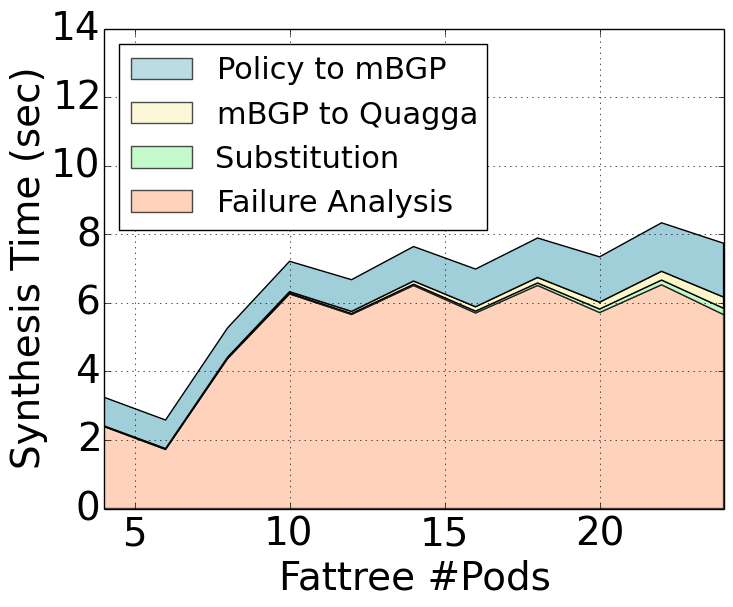
\includegraphics[width=.49\columnwidth]{figures/Fattree-analysis-time.png}}
  \subcaptionbox{Backbone}
    {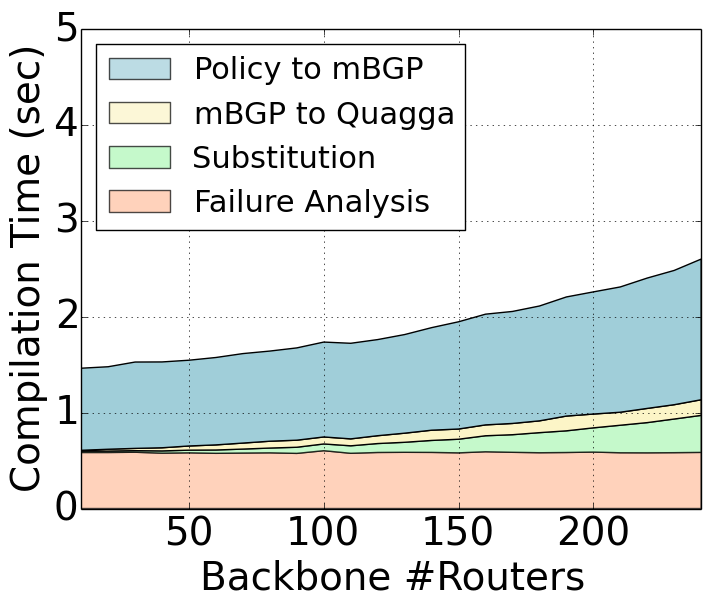
\includegraphics[width=.49\columnwidth]{figures/backbone-analysis-time.png}} \\
  \caption{Abstract Compilation Time by Phase. \label{fig:abstract-breakdown}}
  \vspace{-1em}
\end{figure}

Using abstraction allows us to naturally scale network synthesis in \sysname. We evaluate compilation time in \sysname both with and without abstraction using routing policy for backbone and datacenter networks inspired by configurations obtained from a large cloud provider.

\para{Routing Policy}

Routers in the datacenter network run BGP using private AS numbers and peer with each other and with the backbone network over eBGP. The routers aggregate some prefix blocks when announcing them to the backbone network, and they keep some prefixes internal. The policy also ensures bogons and private address space from external neighbors is dropped. The data center prefers that traffic leave through certain peers over others and ensures that transit traffic between peers is never allowed in the datacenter.

The backbone network classifies external neighbors into several different categories based on commercial relationship and prefers paths through them in order. Similar to the datacenter, it prevents bogons and private address space from external neighbors, drops transit traffic between certain peers but not through others, and aggregates internal prefixes at the border of the network.

\para{Network Topology}

For both networks, we use the same routing policy but scale the size of the underlying topology. For the datacenter networks, we use a standard Fat Tree topology and scale the size of the topology according the the number of pods $k$, starting with 4 pods and ending with 24 pods. The abstract topology uses a single abstract node for each tier of the datacenter, an additional abstract node for tier 0 to separate local and global prefixes, as well as a single abstract node for each group of equivalent eBGP neighbor.

For the backbone networks, we split the network into two parts: a collection of border routers and a fully-connected internal core. We scale the backbone networks from 10 to 250 routers. The abstract topology uses a single abstract node for the network border routers and another abstract node for the network core. Backbone eBGP-speaking peers are grouped into abstract nodes based on their commercial relationship to the current AS (e.g., customer, provider, peer).

\para{Results}

Figure~\ref{fig:compilation-times} shows compilation time for the same policies for both the abstract and concrete versions of the policies described above. All experiments are run on an 8 core, 2.4 GHz Intel i7 processor Mac with 8GB of Ram.

For both the datacenter and backbone networks, the abstract compilation starts off slightly slower than concrete compilation for small topologies due to the overhead of the abstract k-disjoint path analysis for aggregation black-hole safety. However, as the size of the topology increases, abstract compilation becomes orders of magnitude faster than concrete compilation. In all cases for both networks, abstract compilation takes less than 10 seconds to complete.

Figure~\ref{fig:abstract-breakdown} shows the relative time taken by each phase of abstract compilation. Notably, the abstract analysis takes the majority of the time, however the analysis does not depend on the number of concrete nodes in the network, and thus is largely a fixed cost. In particular, the number of calls to $\nu$Z remains constant the across topology size. The seesaw behavior for the data center networks results from differences in time taken by $\nu$Z to minimize the same constraints with different parameters.




%=====================================================
%
%
%  **Related Work**
%
%
%=====================================================

\section{Related Work}
\label{sec:related}

Our work is related to four threads of prior work.

\para{Network synthesis} Many recent systems focus on allowing operators to specify  their policies at a high level. These can be classified into two classes. The first class targets networks based on SDN (software-defined networking) and directly generates the forwarding rules that tell routers how to forward packets~\cite{x,y,z}. The second class, and to which our work belongs, targets conventional networks and generates router configuration, based on which the routers interact and compute forwarding rules~\cite{propane,narain:lisa05,narain+:configassure}. Almost all large networks (old or new) use the conventional paradigm because that scales better~\cite{bgp-in-dc}.

While we borrow much from existing configuration synthesis work, especially Propane~\cite{propane}, our goal is to generate role templates from abstract topologies, rather than router configurations from concrete topologies. This goal aligns better with operators' mental models and tools and permits network evolution with minimal disruption to existing routers. In the process, develop new abstractions for network topologies, fault-tolerance analysis algorithms for abstract topologies, and assign formal semantics to templates.

\para{Topology design} Network topology design, especially for data centers, is another active research area, with researchers exploring designs with different properties~\cite{x,y,z}.  We do not develop new designs but develop abstractions that can capture these designs (and their evolution) and algorithms that can analyze the fault tolerance of abstract topologies. 

While not the focus of this paper, our tools can enable operators to pick the right design for their networks, more quickly and with stronger guarantees. Today, when picking the design, operators analyze its multiple concrete instantiations because available analysis tools only work with concrete topologies~\cite{condor}. This process is time-consuming and not fool-proof; analyzing large, concrete topologies (with potentially thousands of nodes) takes a lot of time and the analysis does not cover the entire space of topologies that may arise.

\para{Network verification}
A complementary approach to reducing configuration errors is by analyzing the forwarding rules or configuration of the network to ensure the absence of (a class of) bugs~\cite{anteater,hsa,feamster+:rcc,ipassure,batfish,bagpipe,arc,era,symmetries}. Our focus, in contrast, is on a correct-by-construction approach. It has the downside that operators must learn to express policies in a new language, but it saves them from the challenging and time-consuming task of configuration generation and provides stronger guarantees on correctness.


%\para{Configuration synthesis}
%ConfigAssure~\cite{narain:lisa05,narain+:configassure}
%is another system designed to
%help users define and debug low-level router
%configurations.  Inputs to
%ConfigAssure include a \emph{configuration database}, which contains a
%collection of tuples over constants and configuration variables, and a
%\emph{requirement}, which is a set of constraints.
%%
%The authors use a combination of logic programming and
%SAT solving to find concrete values for configuration variables.
%ConfigAssure handles configuration for a wide range of protocols and many
%different concerns.  In contrast, the scope of \sysname is much
%narrower.  In return, \sysname offers compact, higher-level
%abstractions customized for our domain, such as regular paths, as well
%as domain-specific analyses customized to those abstractions, such as
%our failure safety analysis.  The implementation technology is also
%entirely different, as we define algorithms over automata and graphs
%as opposed to using logic programming and SAT-based model-finding.



%=====================================================
%
%
%  **Conclusions**
%
%
%=====================================================

\section{Conclusions}
\label{sec:conclusions}

To help configure large networks correctly, we develop \sysname, the first system that can generate role templates from high-level specifications of network topology and policy. \sysname is based on new abstractions for capturing network topologies, and their evolution, and algorithms to analyze the combined impact of topology and routing policy on the network's fault tolerance. Our analysis operates entirely in the abstract domain and guarantees correctness for all concrete instantiations of the topology. Experiments with many types of real-world topologies and policies show that our abstractions and analysis are precise and that, for large networks, configuration synthesis is two orders of magnitude faster than systems that operate over concrete topologies.


%=====================================================
%
%
%  **Bibliography**
%
%
%=====================================================

\balance


\bibliographystyle{abbrvnat}
\bibliography{references}


%=====================================================
%
%
%  **Appendix**
%
%
%=====================================================


\end{document}
